\documentclass[12pt,a4paper,twoside]{book}
\usepackage[english]{babel}
\usepackage{graphicx}
\usepackage{amsmath}
\usepackage[font=small,labelfont=bf]{caption}
\newcommand{\norm}[1]{\lVert#1\rVert}

\bibliographystyle{abbrv}
\begin{document}

\begin{titlepage}
  \begin{center}
    \begin{Large}Universit\`a degli Studi di Trento\\\end{Large}
     Facolt\`a di Scienze Matematiche, Fisiche e Naturali\\
     \vspace{10pt}
     \begin{figure}[htbp]
       \begin{center}
         
\includegraphics[width=3cm]{images/sigillo_unitn.eps}
       \end{center}
     \end{figure}
Corso di Laurea in Informatica\\

\vspace{10pt}
\line(1,0){338}
\vspace{10pt}

Final Thesis\\
\end{center}
\vspace{3cm}
\begin{center}
\begin{Large}Analysis and implementation of a particle-based model for skiing traffic\\\end{Large}
\vspace{3cm}
\end{center}
Relatore interno: \\ \textbf{Prof. Alberto Montresor} \\
Relatore esterno:\hspace{6.8cm}Laureando:   \\
\textbf{Dott. Cesare Furlanello}\hspace{4.9cm}\textbf{Matteo Poletti}
\vspace{1cm}
\begin{center}
Anno accademico 2012-2013
\end{center}
\end{titlepage}
\tableofcontents
\chapter*{Introduction}
\addcontentsline{toc}{chapter}{Introduction}


%%%%%%%%%%%%%%%%%%%%%%%%%%%%%%%%%%%%%%%%%%%%%%%%%%%%%%%%%%%%%%%%%%%%%%%%%%%%%%%%%%%%%%%%
\chapter{The model}\label{model}
The model implemented describes a two-dimensional microscopic-driven many-particle system. Published by Holleczek and Troster \cite{hol2012} it is based on the constraint that skiers are exposed to gravity and centripetal forces.
.
Skiers are modeled as particles with a specific mass, $m$, that are exposed to two class of forces: 
1)social forces that determine skiers behavior. 
2)Physical forces, that regulate the skier motion determining the acceleration. 
The position of a skier at time $t$ is represented by the following vector $r(t)$, $\dot{r}(t)=\frac{d}{dt}r(t)$ its speed, and $e_{\dot{r}}(t)=\ \dot{r}(t) / \Vert \dot{r}(t)\Vert$ that defines the direction of motion.

\section{Social forces}
The social forces implemented in the model describe the decisions taken by a skier while descending a slope. Social forces are dimensionless and are used to determine whether the skier should take a turn or not, however they do not act on acceleration. The superposition of all social forces, $F_{social}$, gives skier's desired direction  $e_{social}(t)=F_{social} / \Vert F_{social} \Vert$. If the desired direction $e_{social}(t)$ diverges from the actual skier direction of motion $e_{\dot{r}}(t)$ more than an angle ${\delta}$, the skier starts to turn adjusting the direction (see Fig.\ref{start_turn_pic}). Social forces are used to model the repulsion of the skier from slope edges, potential obstacles and from other skiers on the other side these forces attract skiers towards the destination chosen.

\begin{figure}[!ht]
  \begin{center}
    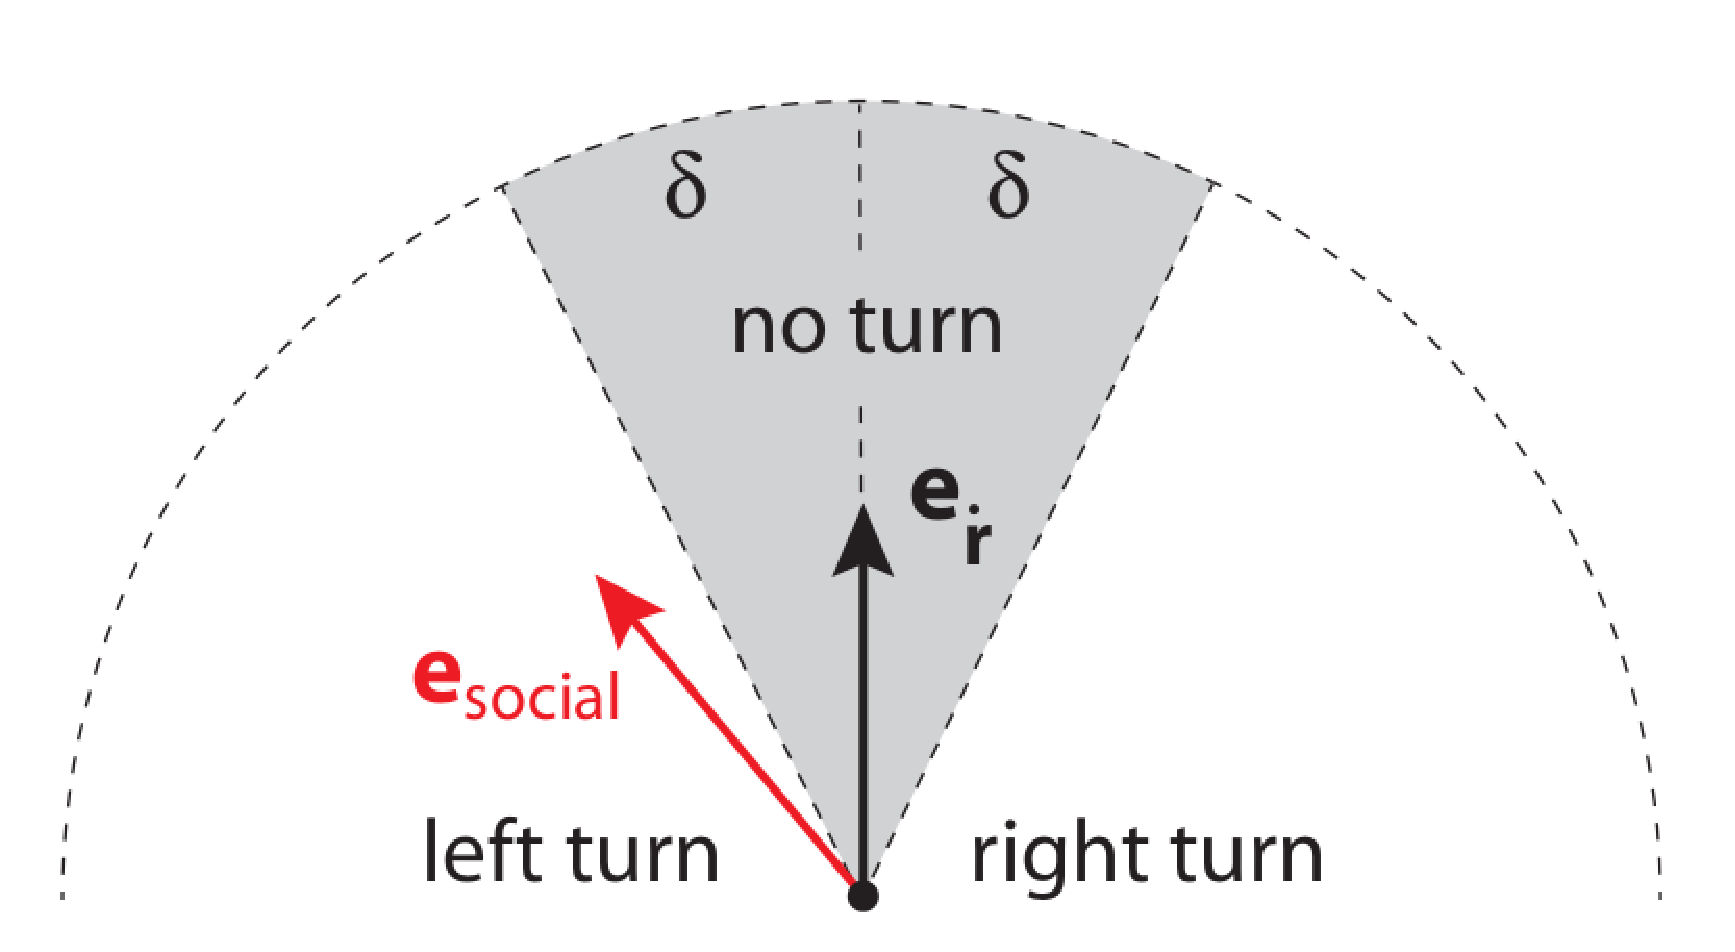
\includegraphics[width=0.4\textwidth]{images/start_turn_pic.eps}
    \caption{(From \cite{hol2012}) When the angle between the current direction of motion $e_{\dot{r}}$ and the desired direction $e_{social}$ is bigger than $\delta$ the skier performs a turn to adjust his or her direction}\label{start_turn_pic}
  \end{center}
\end{figure}

To describe the social force that attracts the skier towards the chosen destination, the model assumes that each skier, while descending, selects several waypoints $x_a^1....x_a^n$ as temporary destinations. Thus, at each time $t$ the skier $a$ wants to reach a waypoint $x_a^k$. The direction toward the current waypoint is expressed by

\begin{equation}\label{waypoint_direction}
e_a(t)=\frac{x^k_a-r_a(t)}{\Vert x^k_a-r_a(t) \Vert}
\end{equation}
where, as defined above, $r_a(t)$ is the position of $a$ at time $t$. The destination social force drives the skier toward the waypoint and is as follows

\begin{equation}\label{destination_force}
F_D(r_a)=A_0 e_a(t)
\end{equation}
where $A_0$ is a scaling constant that represents the strength of the destination force.

The attitude of skiers to keep a minimum distance from the edges is modeled with repulsion forces that are stronger when the skier gets closer to the edge of the slope. At each position $r_a$ the skier $a$ is subjected to a repulsion force from the left edge of the slope and to a repulsion force from the right edge of the slope. Let $r_a^L$ be the closest location to $r_a$ on the left edge, then the distance between the skier and the edge can be expressed as $r_{aL}=r_a-r_A^L$. The repulsion force from the left edge is defined as

\begin{equation}\label{left_force}
F_L(r_{aL})=-\nabla_{r_{aL}}U(\Vert r_{aL} \Vert )
\end{equation}
where $U(\Vert r_{aL} \Vert )$ is a monotonically decreasing potential. In a symmetric way the repulsion force from the right edge can be defined as

\begin{equation}\label{right_force}
F_R(r_{aR})=-\nabla_{r_{aR}}U(\Vert r_{aR} \Vert )
\end{equation}
The model takes into account also the natural human behavior of avoiding collisions with other skiers. This is described by a repulsion force, referred as skier repulsion force, that each skier imposes on the other skiers. The repulsion force that skier $b$ imposes on the skier $a$ can be expressed as

\begin{equation}\label{skier_force}
F_S(r_{ab})=-\nabla_{r_{ab}}V(s(r_{ab}))
\end{equation}
where $r_{ab}=r_a-r_b$ is the distance vector between the two skiers, $V(s(r_{ab}))$ is a monotonically decreasing potential with equipotential lines shaped as ellipses directed into the direction of motion and $s$ represents the semiminor axis of this ellipse and is defined as

\begin{equation}\label{skier_s}
s(r_{ab})=\frac{\sqrt{(\Vert r_{ab} \Vert + \Vert r_{ab}-v_b \Delta t e_b \Vert )^2-(v_b \Delta t)^2}}{2}
\end{equation}
Finally a repulsion force from the obstacles on the slope is considered. The force that an obstacle $o$ imposes on the skier $a$ is defined as

\begin{equation}\label{obstacle_force}
F_O(r_{ao})=-\nabla_{r_{ao}}W(\Vert r_{ao} \Vert )
\end{equation}
In general, repulsion social forces act on skiers only if he or she is capable of perceiving what triggers the force. The model assumes that objects are perceived only within a certain range $\varphi$ of the skier direction. $2\varphi$ can be considered as the angle of view. This is modeled by the weight

\begin{equation}\label{visibility}
w(u,v)=\begin{cases}
  1 & \text{if $(u/\Vert u \Vert)\cdot (v/\Vert v \Vert) \geq cos \varphi$} \\
  0 & \text{otherwise }
  \end{cases}
\end{equation}
To summarize, social forces modeled for every skier $a$ are
\begin{align}\label{social_forces_tb}
F_D(r_a)&=A_0 e_a(t),\\
F_L(\dot{r_a},r_{aL})&=w(\dot{r_a},-r_{aL})F_L(r_{aL}),\\
F_R(\dot{r_a},r_{aR})&=w(\dot{r_a},-r_{aR})F_R(r_{aR}),\\
F_A(\dot{r_a},r_{ab})&=w(\dot{r_a},-r_{ab})F_A(r_{ab}),\\
F_O(\dot{r_a},r_{ao})&=w(\dot{r_a},-r_{ao})F_O(r_{ao})
\end{align}

The resultant social force $F^a_{social}$ is the superposition of all social forces that apply on skier $a$:

\begin{equation}
F^a_{social}=F_D(r_a)+F_L(\dot{r_a},r_{aL})+F_R(\dot{r_a},r_{aR})+\sum_b F_A(\dot{r_a},r_{ab})+\sum_o F_O(\dot{r_a},r_{ao})\nonumber
\end{equation}
Figure \ref{social_forces_diagram} shows a diagram of the social forces described above.

\begin{figure}[!ht]
  \begin{center}
    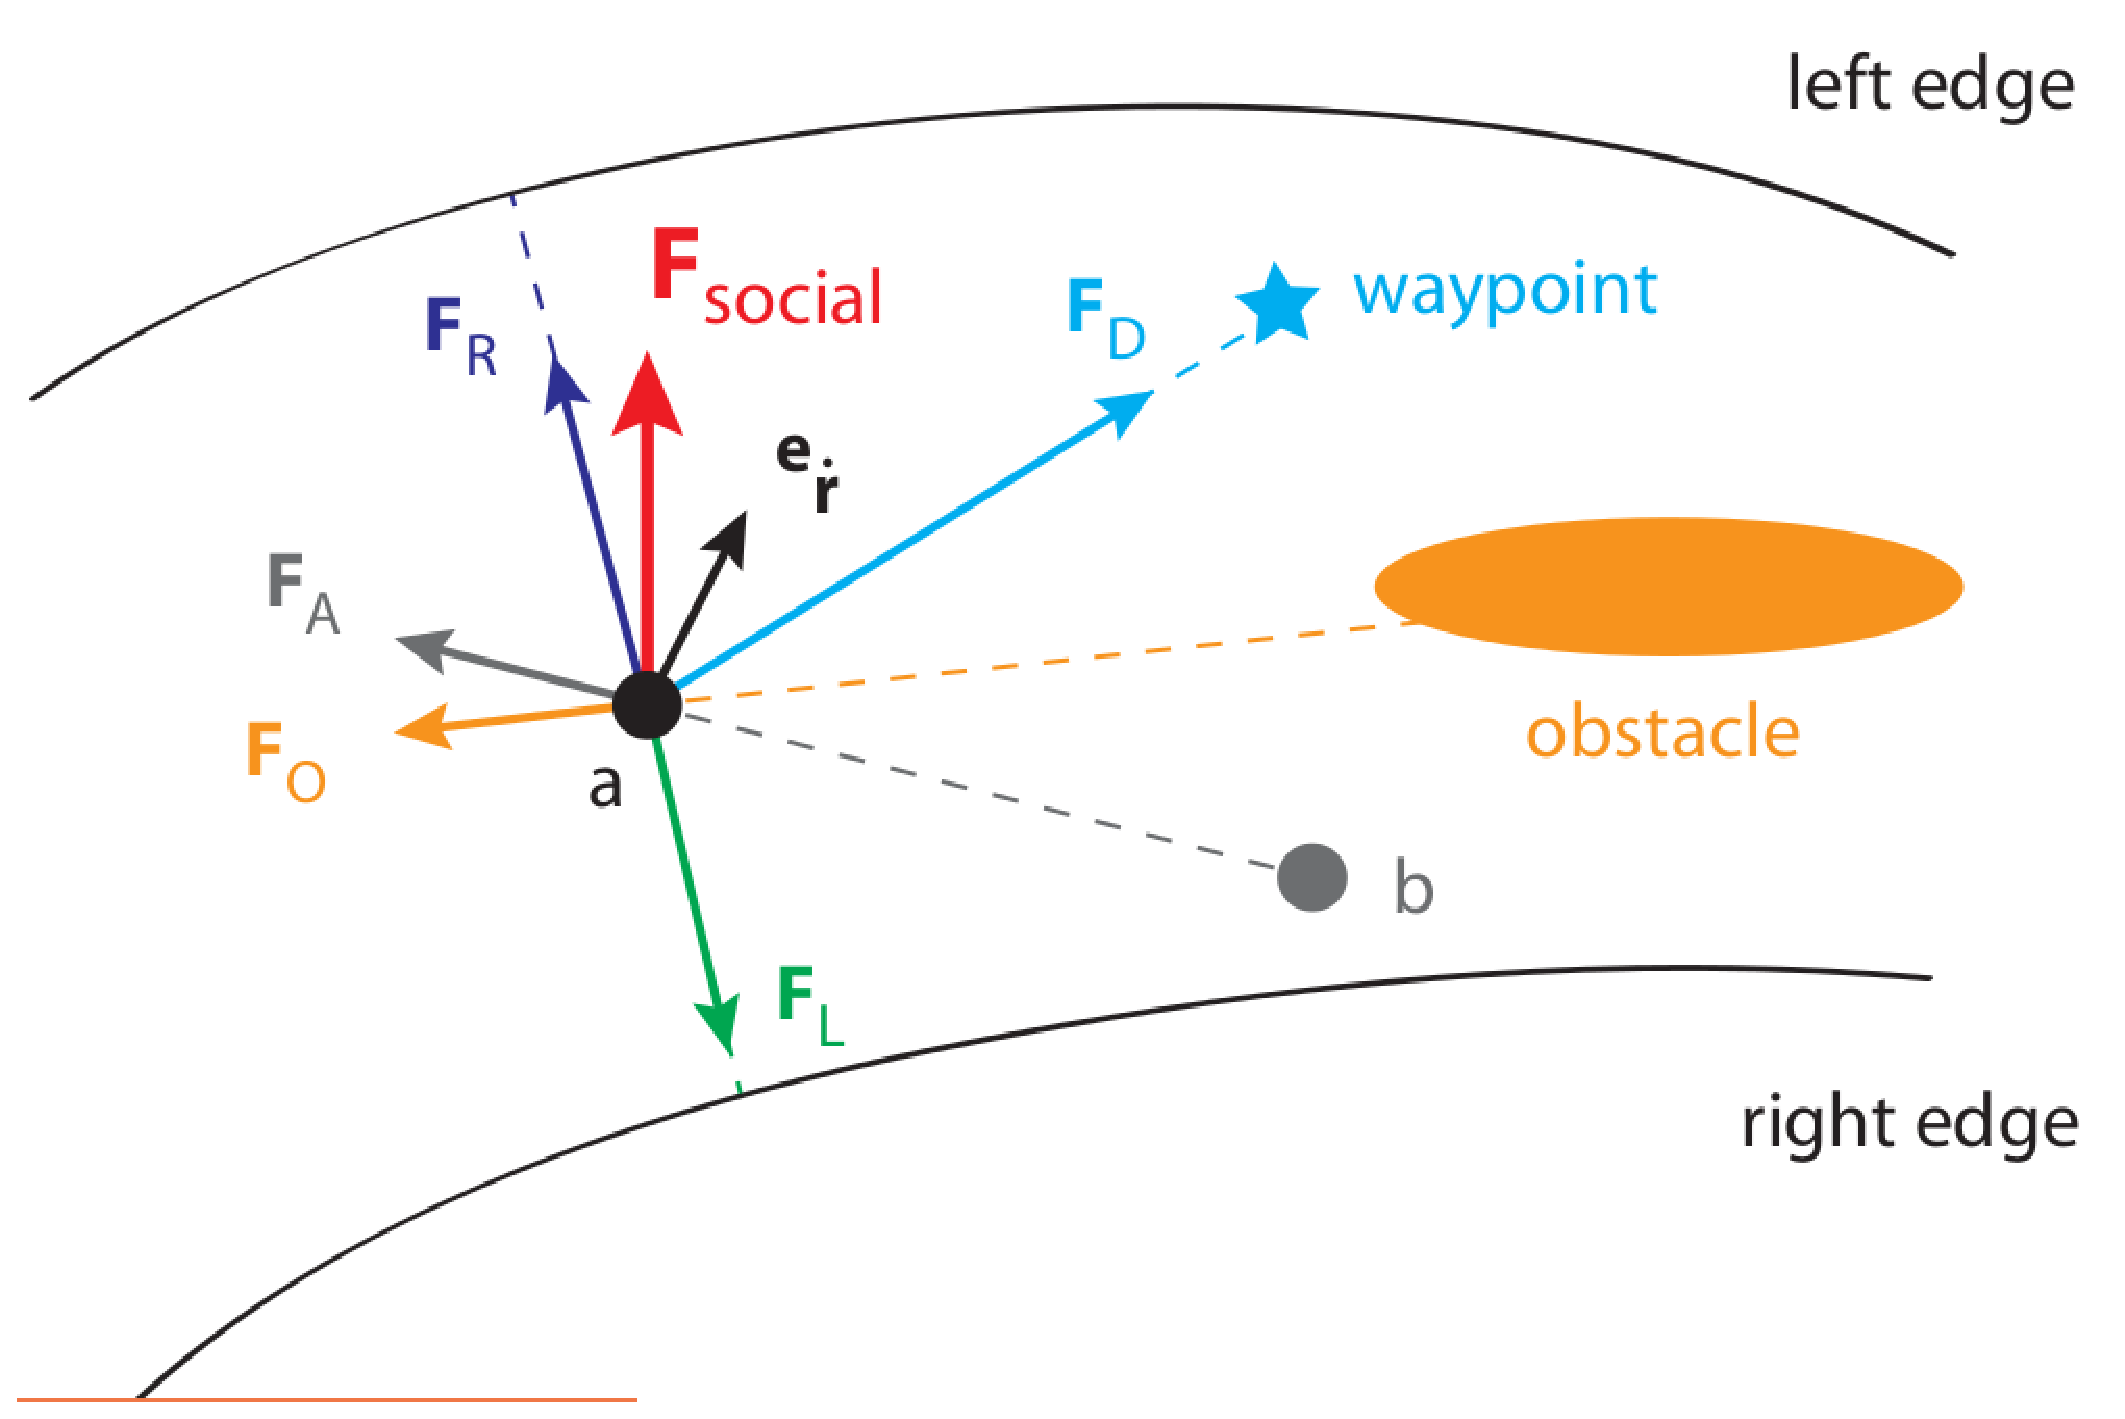
\includegraphics[width=0.8\textwidth]{images/social_forces_dia.eps}
    \caption{Diagram of the social forces. The forces $F_R$ and $F_L$ keep the skier $a$ away from the edges, the force $F_O$ repels the skier from the obstacle, the force $F_S$ repels $a$ from the skier $b$ and the force $F_D$ attracts the skier towards the waypoint.}\label{social_forces_diagram}
  \end{center}
\end{figure}


\section{Physical forces}
As described in \cite{hol2012}, there are two major techniques used to curve while skiing: \textit{skidding} and \textit{carving}. When carving, the direction of motion is exclusively parallel to the skis while in skidding there is an additional slippage to the side. Carved turns are usually performed by expert skiers, while beginners and not experienced skiers tend to perform skidded turns.

In \cite{hol2012} skiers are supposed to perform turns with a radius corresponding to the \textit{sidecut radius} of their skis. Although some studies \cite{jen2004} \cite{fe2010} have proposed a more realistic model of carving turns,deeply investigating the effects of ski penetration  in the snow and of the skier tilt angle, as a first version of the model the approximation of the turning radius to the sidecut radius has been considered acceptable. Figure \ref{sidecut_radius} shows the relation between sidecut radius and turning radius.

\begin{figure}[!ht]
  \begin{center}
    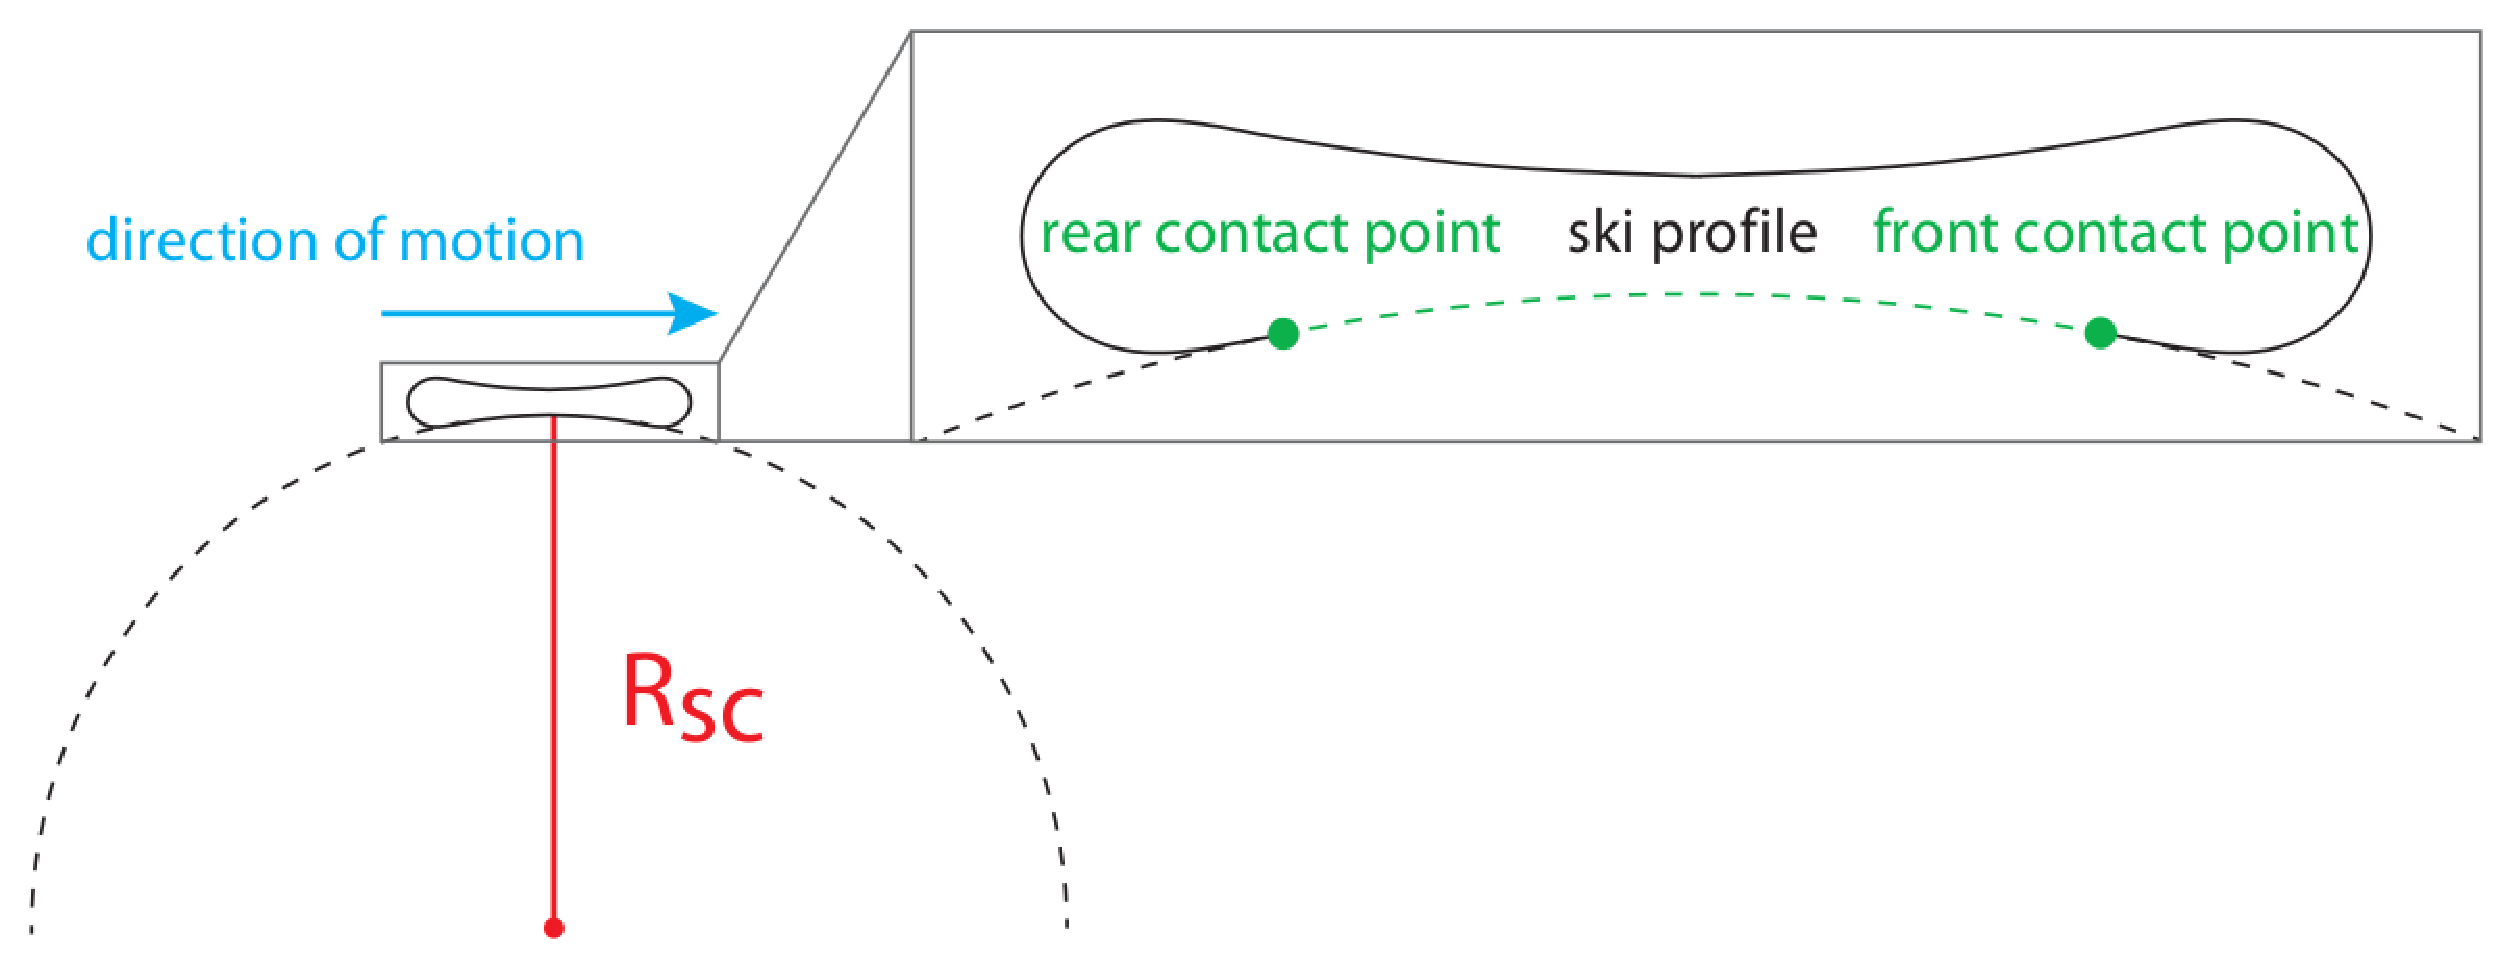
\includegraphics[width=0.8\textwidth]{images/sidecut_radius.eps}
    \caption{(from \cite{hol2012}) Profile of a carving sking with the sidecut radius and the turning radius evidenced.}\label{sidecut_radius}
  \end{center}
\end{figure}

Gravitational, centripetal and friction forces determine the skier acceleration according to their direction $e_{\dot{r}}$. Consider a skier at position $r$ with speed $\dot{r}$ and direction of motion $e_{\dot{r}}$ and let $n$ denote the surface normal on the ski slope at $r$. At $r$, the slope has an inclination angle of

\begin{equation}
\alpha =\arccos(\left[0,0,1\right] \cdot n)
\end{equation}
and the inclination angle $\gamma$ of the current trajectory $e_{\dot{r}}$ is

\begin{equation}
\gamma =\arcsin[(\sin \alpha )(\sin \beta )]
\end{equation}
where $\beta$ is the angle between $e_{\dot{r}}$ and the horizontal of the slope.

To compute the force accelerating the skier the gravitational force, the friction forces and the centripetal forces should be investigated. As first the gravitational force $F_G$ is considered. It can be expressed as

\begin{equation}
F_G=mg\left[\begin{matrix}0\\0\\-1\end{matrix}\right]
\end{equation}
where $g$ is the gravitational acceleration and $m$ the mass of the skier. The gravitational force can be subdivided into normal force $F_N$, acting parallel to the surface normal $n$, and into downhill force $F_S$, acting parallel to the fall line.

\begin{equation}\label{downhill_force}
F_G=F_S-F_N
\end{equation}
The normal force $F_N$ can be expressed as
\begin{equation}
F_N=mg(\cos \alpha )n
\end{equation}
The  downhill force $F_S$ itself can be subdivided into $F_P$ which is acting parallel to the current trajectory $e_{\dot{r}}$ and into the lateral force $F_{lat}$ acting perpendicularly to the current trajectory (see. Fig\ref{downhill_force_pic}).

\begin{equation}
F_S=F_P+F_{lat}
\end{equation}
\begin{figure}[!ht]
  \begin{center}
    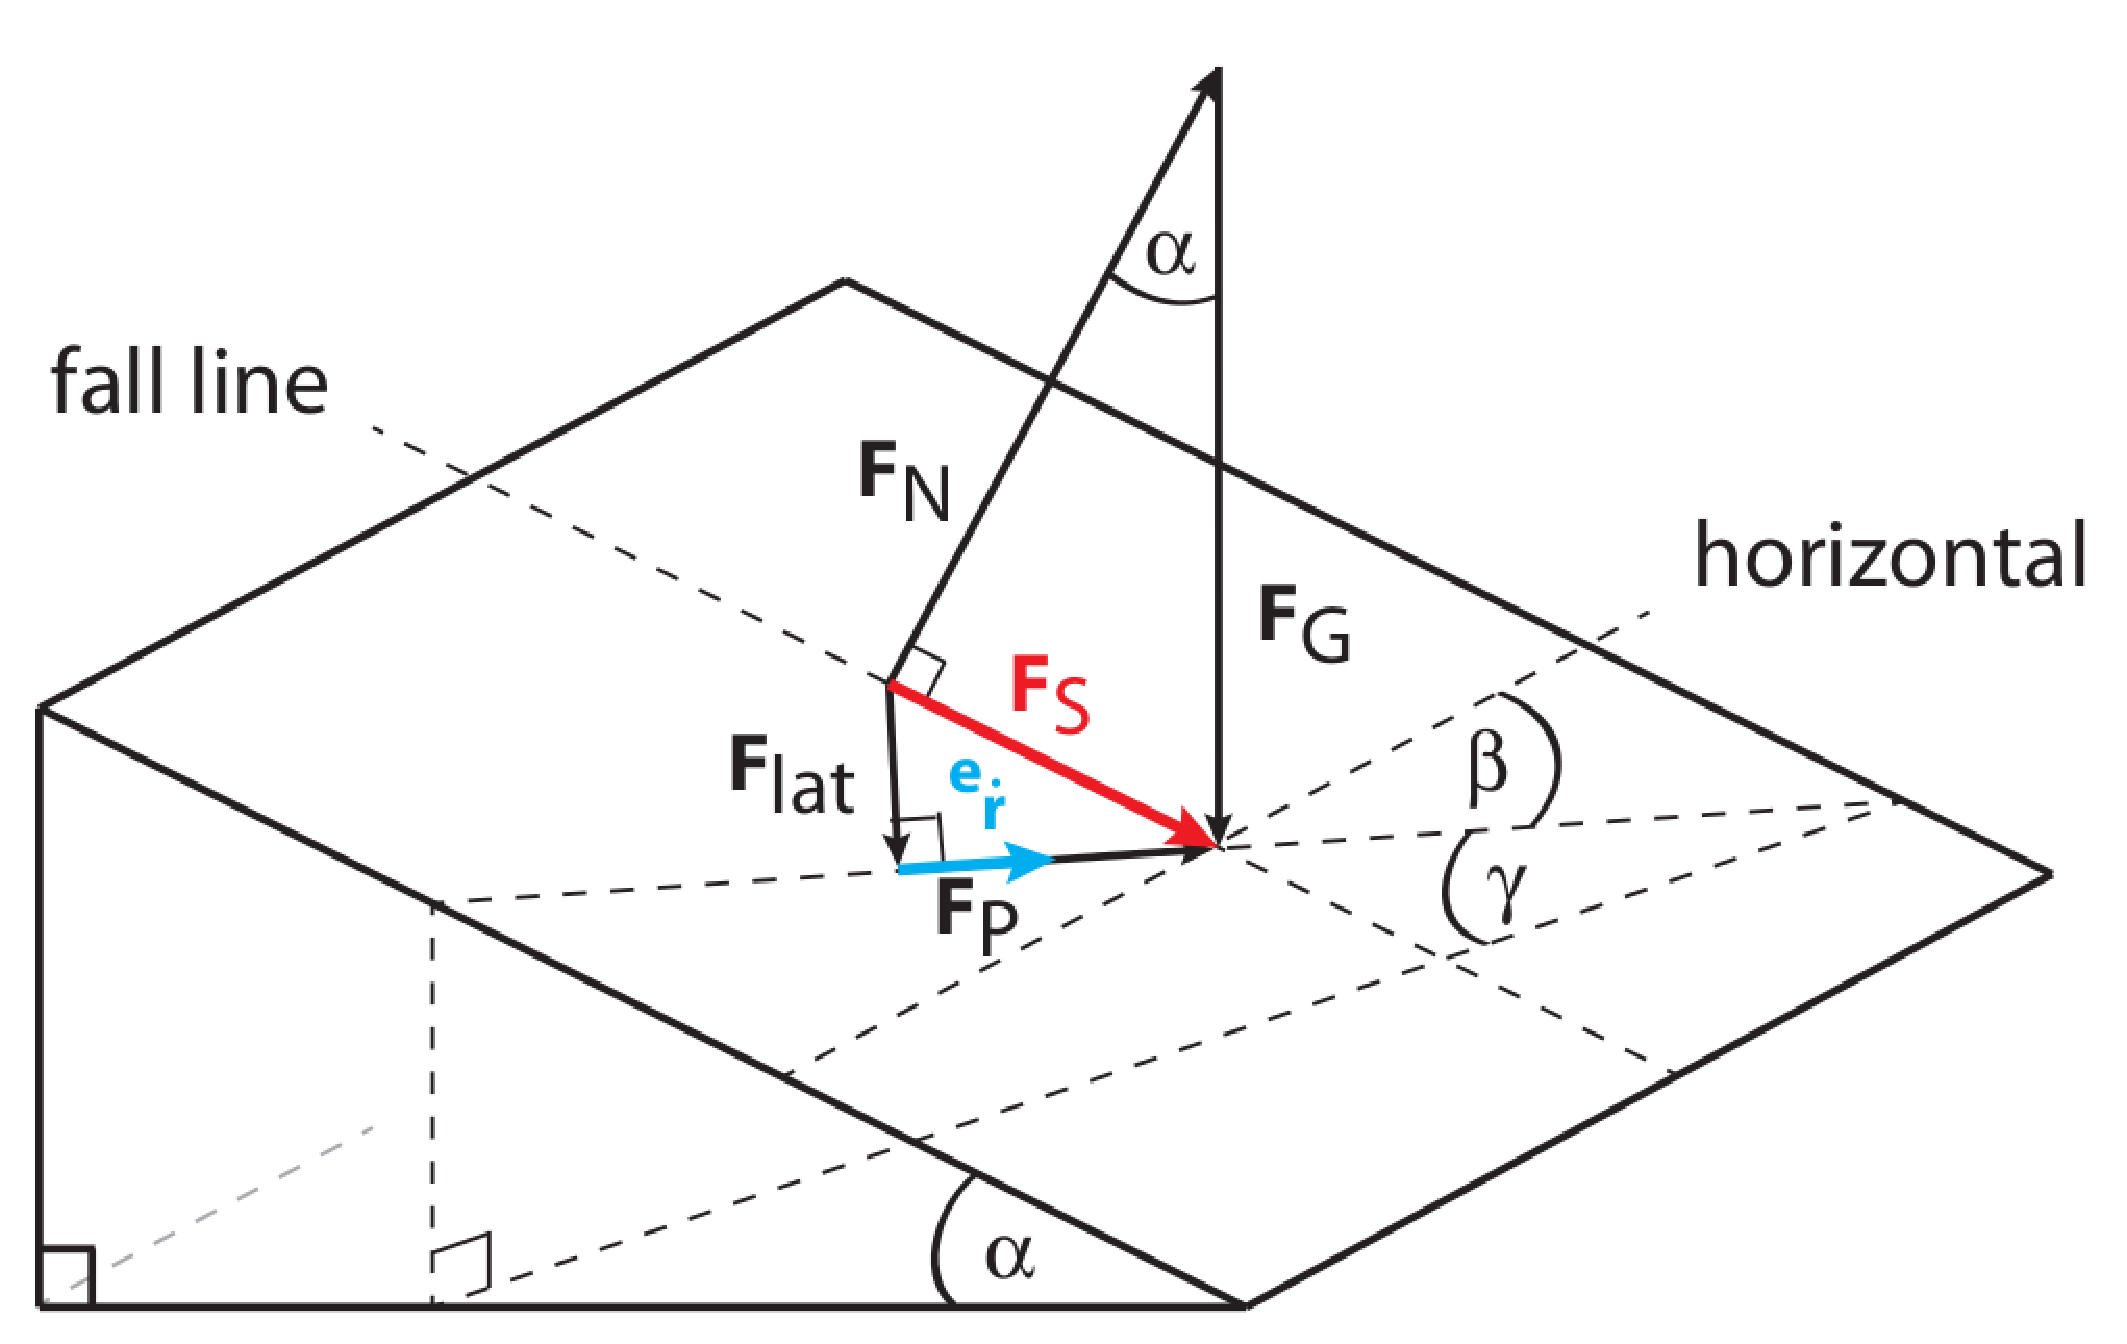
\includegraphics[width=0.5\textwidth]{images/figure5.eps}
    \caption{(from \cite{hol2012}) The downhill force $F_S$ can be decomposed into the downhill force $F_P$, acting parallel to the current trajectory, and into the lateral force $F_{lat}$ acting perpendicularly to the direction of travel.}\label{downhill_force_pic}
  \end{center}
\end{figure}

The downhill force $F_p$ can be written as
\begin{equation}
F_P=mg ( \sin \gamma ) e_{\dot{r}}=mg ( \sin \alpha ) ( \sin \beta ) e_{\dot{r}}
\end{equation}
where $\gamma$ is the inclination angle of $e_{\dot{r}}$.

Remembering \ref{downhill_force}, the downhill force $F_S$ can be computed as
\begin{equation}
F_S=F_G+F_N
\end{equation}
The lateral force $F_{lat}$ can therefore be computed as

\begin{equation}
F_{lat}=F_S-F_P
\end{equation}
The centripetal force $F_C$ a skier is exposed while turning can be written as

\begin{equation}
F_C=\frac{m}{R_{SC}} {\norm{\dot{r}}}^2 \frac{F_{lat}}{\norm{F_{lat}}} \times
\begin{cases}
  (+1) & \text{before crossing the fall line} \\
  (-1) & \text{after crossing the fall line}
  \end{cases}
\end{equation}
where $m$ is the mass of the skier and $R_{SC}$ the sidecut radius of the skis. $F_C$ is parallel to $F_{lat}$ before the skier crosses the fall line and antiparallel to $F_{lat}$ after having crossed the fall line.

Before defining the kinetic friction of skis on snow, a definition of effective force should be given. The effective force is the force that needs to be compensated by the snow. Its formulation depends on whether the skier is performing a turn or is descending on a straight line. In the following, when the definition of a force changes depending on whether the skier is turning, the index is written lowercase in the case of a straight line and uppercase in the case of a turn. So $F_{eff}$ is the effective force acting on a skier that is descending on a straight line and is defined as

\begin{equation}
F_{eff}=F_{lat}-F_N
\end{equation}
If the skier is performing a carved turns then the effective force $F_{EFF}$ can be written as

\begin{equation}
F_{EFF}=F_{lat}-F_C-F_N
\end{equation}
Figure \ref{effective_force_pic} shows the effective force ($F_{eff}$ and $F_{EFF}$).

\begin{figure}[!ht]
  \begin{center}
    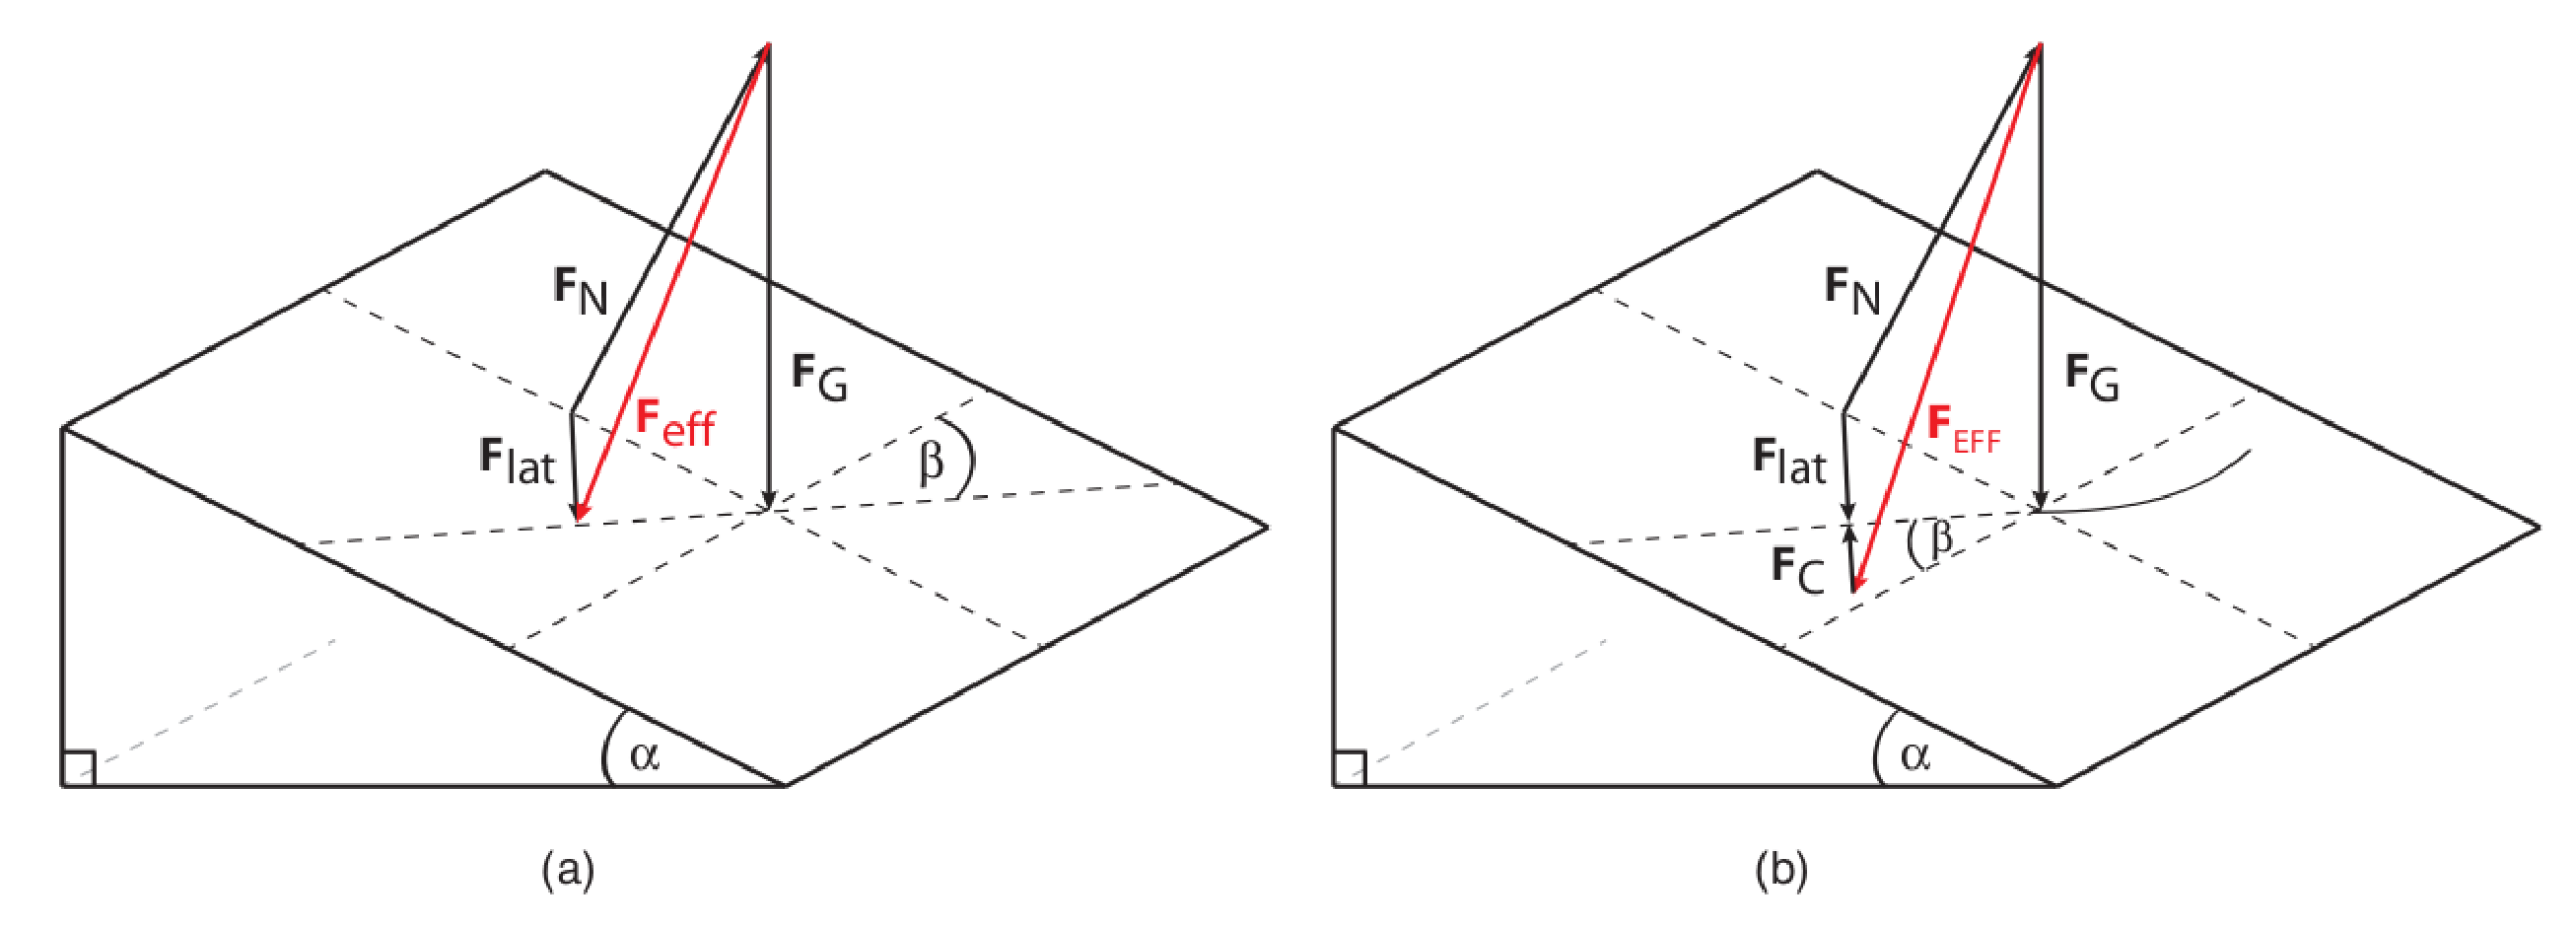
\includegraphics[width=\textwidth]{images/figure6.eps}
    \caption{(from \cite{hol2012}) In (a) effective force during the descent on a straight line ($F_{eff}=F_{lat}-F_N$). In (b) effective force during a carved turn ($F_{EFF}=F_{lat}-F_N-F_C$)}\label{effective_force_pic}
  \end{center}
\end{figure}

The kinetic friction force $F_{ground}$ can be expressed in terms of the skier's effective force as

\begin{equation}
F_{ground}=-\mu \norm{F_{eff}}e_{\dot{r}}
\end{equation}
when descending on a straight line. $\mu$ is the kinetic friction coefficient of the skis on the snow. In case of a turn

\begin{equation}
F_{GROUND}=-\mu \norm{F_{EFF}}e_{\dot{r}}
\end{equation}

The air drag force $F_{air}$ is antiparallel to the direction of motion $e_{\dot{r}}$ and is defined as

\begin{equation}
F_{air}=-\frac{1}{2}C_d \rho A \norm{\dot{r}}^2 e_{\dot{r}}
\end{equation}
where $C_d$ is the drag coefficient, $\rho$ the air density and $A$ the projected frontal area of the skier perpendicular to the direction of motion.

Finally, the net force $F_{net}$ accelerating the skier can be defined as

\begin{equation}
F_{net}=-F_P + F_{air} + F_{ground}
\end{equation}
if the skier is not turning. Otherwise the force is defined as

\begin{equation}
F_{NET}=-F_P + F_{AIR} + F_{GROUND} + F_C
\end{equation}

\section{Limitations}
The model proposed describes the motion of an expert skier that skies performing perfect carved turns and the turning radio is taken constant and equals to the sidecut radius of the skis. Not experienced skiers and other snow-sport athletes are not considered. An important limitation of the model is that it does not consider that skiers could stop while descending a slope.  Moreover skiers are not allowed to jump nor to exit the ski slope. If a skier collides with an edge of the slope it is reflected back with an angle equals to the angle at which he or she has collided.

\section{New features implemented and differences from the original model}
The physical model of the skiers motion has been keep equals to the one exposed in \cite{hol2012}. Within the social forces, the destination force $F_D$ (see. \ref{destination_force}) is of critical importance. The effectivness of this destination force is strongly related to the waypoints selection. In the original paper the waypoints were selected randomly every 50m, using a uniform distribution on the corresponding line from the left to the right edge of the slope (see Fig.\ref{waypoints_old_pic}).

\begin{figure}[!ht]
  \begin{center}
    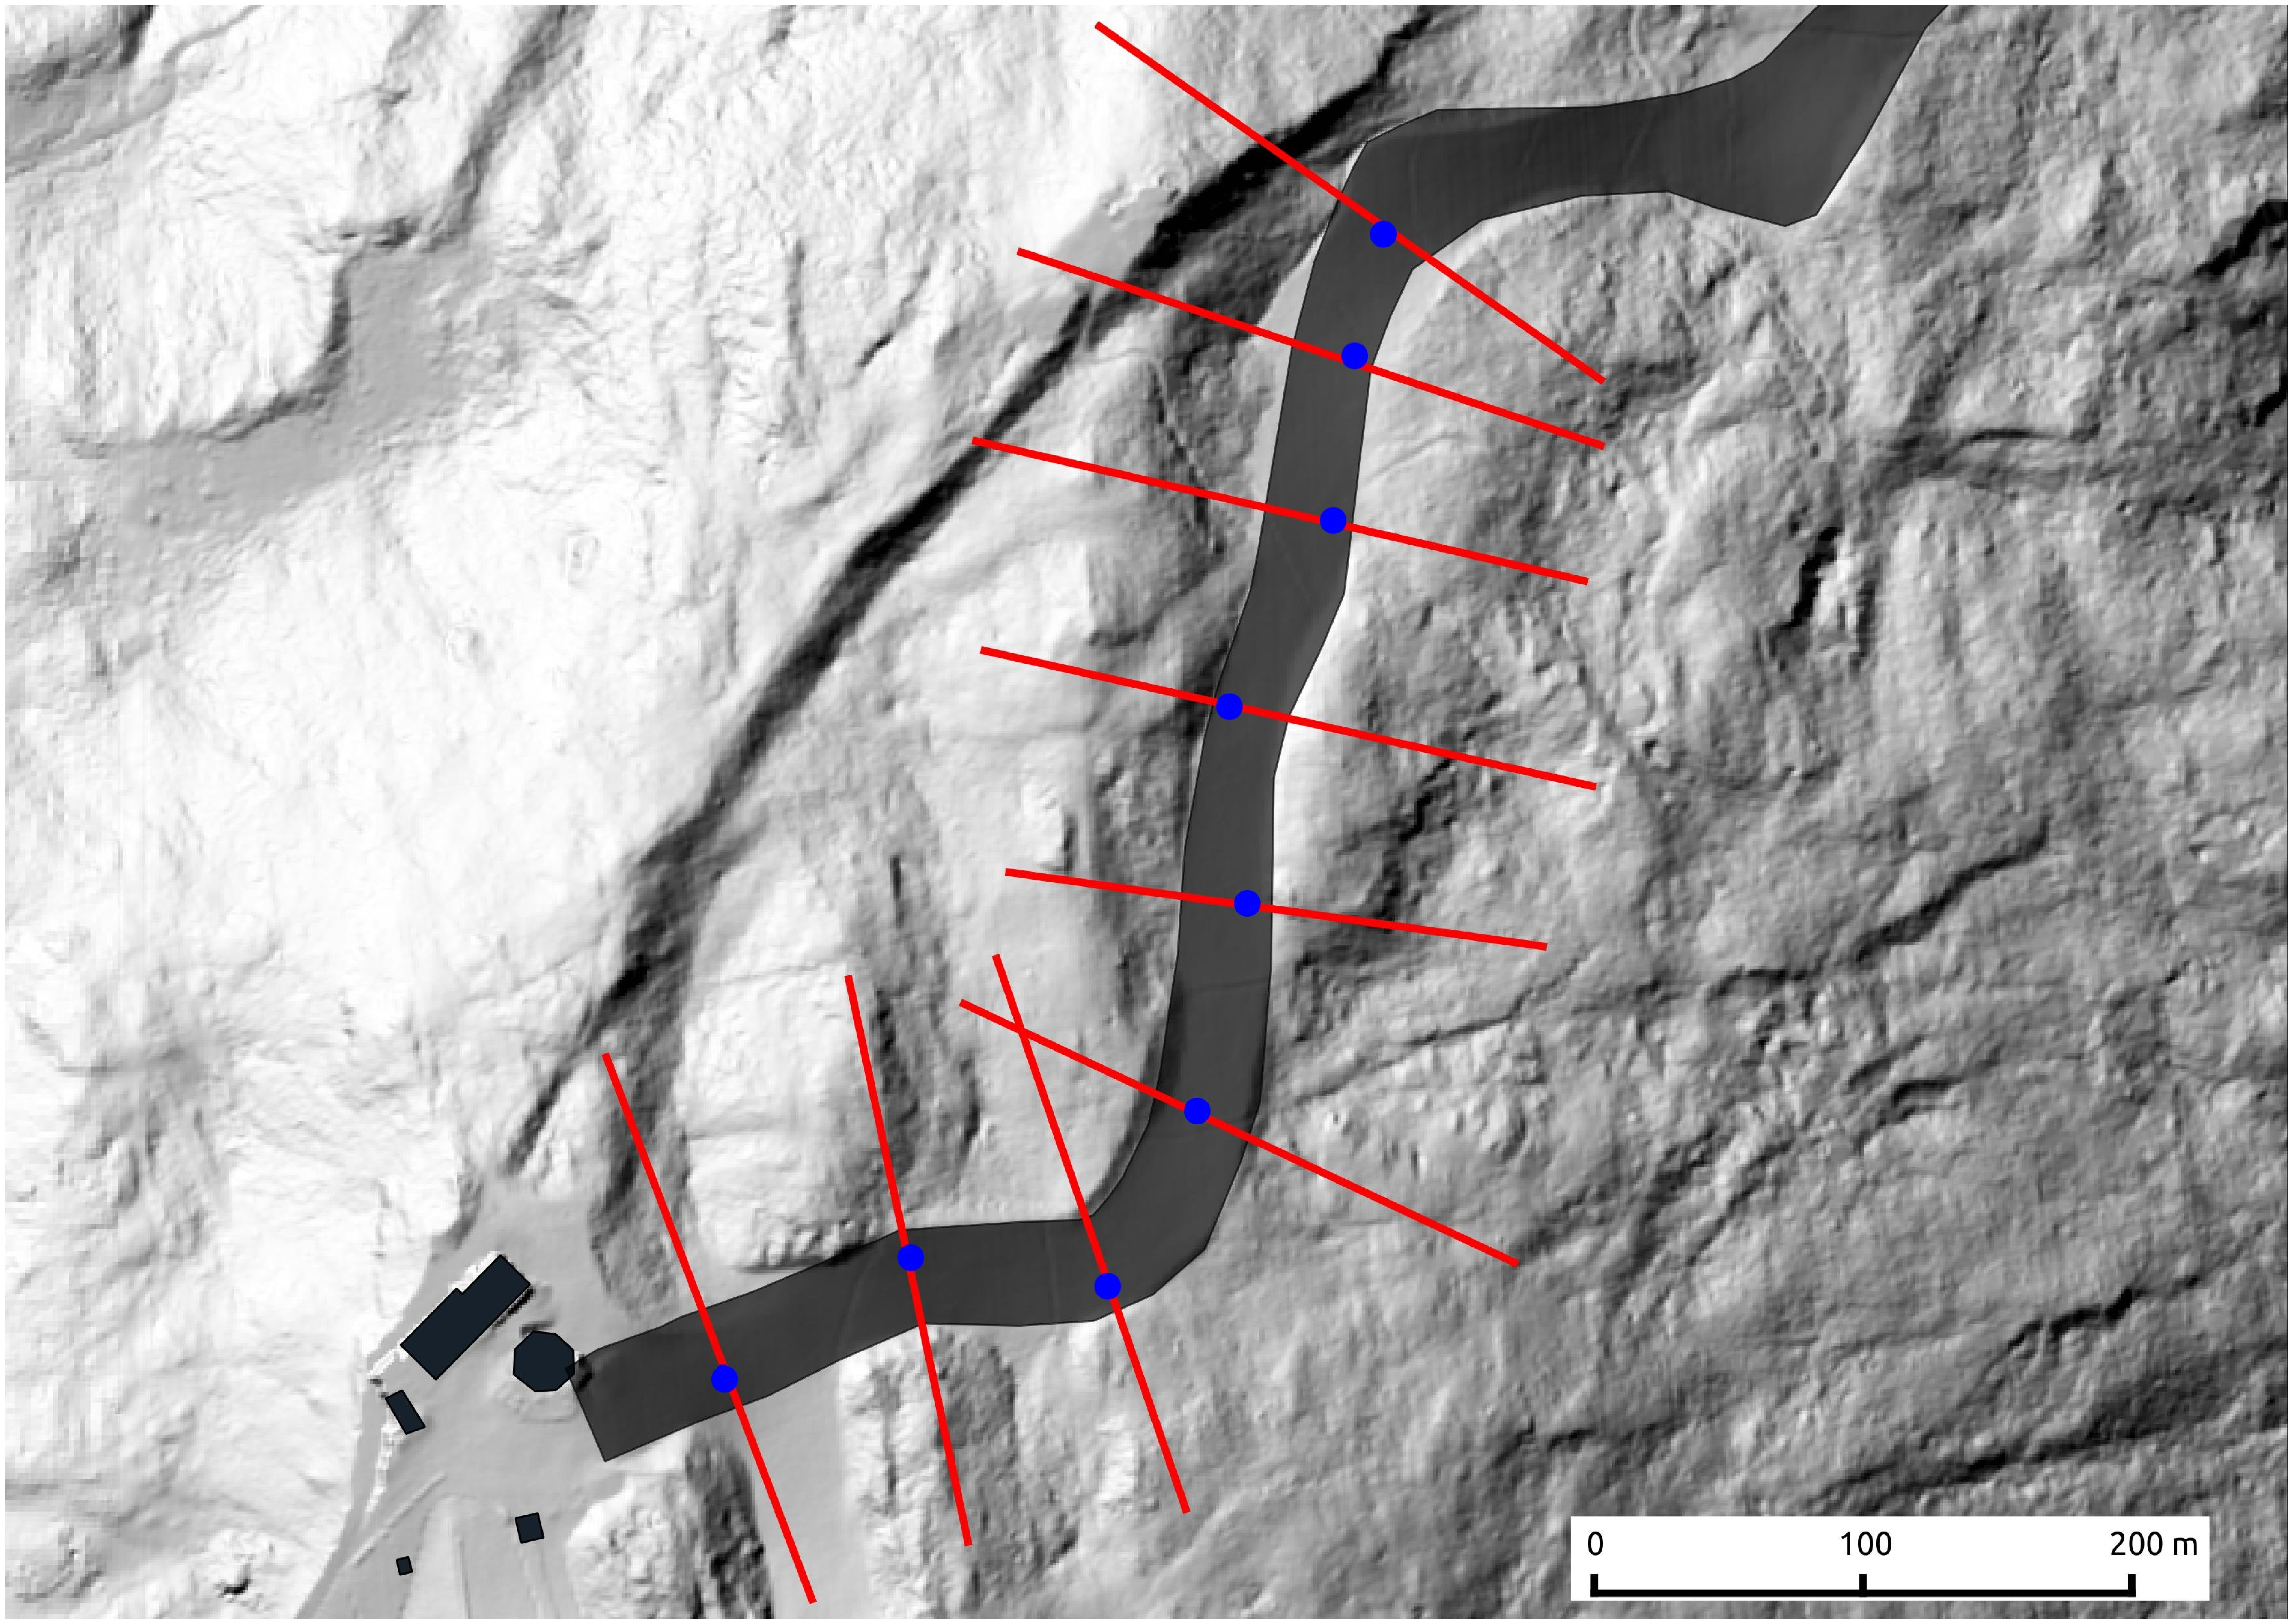
\includegraphics[width=\textwidth]{images/waypoint_line.eps}
    \caption{In \cite{hol2012} waypoints were selected randomly every 50m following a uniform distribution on the line from the left to the right edges of the slope.}\label{waypoints_old_pic}
  \end{center}
\end{figure}

A more dynamic approach in the waypoints selection has been considered to better model the decisions taken from a skier while descending a slope. The new strategy allow each skier to dynamically choose waypoints during the descent, based on the position of the skier, on the shape of the trail, on the slope of the terrain and on the skier speed.

Hereafter the new mechanism for the waypoints selection is explained. Let $a$ be a skier at position $r_a$, let $r_a^L$ be the location on the left slope edge closest to $r_a$ and $r_a^R$ the location on the right slope edge closest to $r$. The vectors given the direction toward the edges are $e_{aR}=\left(r_a^L-r_a\right)/\norm{r_a^L-r_a}$ and $e_{aL}=\left(r_a^R-r_a\right)/\norm{r_a^R-r_a}$. Let $\alpha$ be the angle between $e_{aR}$ and $e_{aL}$ defined as

\begin{equation}
\alpha=\begin{cases}
  \arccos(e_{aR} \cdot e_{aL}) & \text{if(($e_{aR} \times e_{aL})\cdot n \ge 0$)} \\
  2\pi-\arccos(e_{aR} \cdot e_{aL}) & \text{if(($e_{aR} \times e_{aL})\cdot n < 0$)}
\end{cases}
\end{equation}
where $n$ is the normal of the plane containing $e_{aR}$ and $e_{aL}$. The skier $a$ chooses the new waypoint with uniform distribution on a fraction of the angle $\alpha$. More precisely, let $\delta$ be the fraction of angle that should be considered, then the new waypoint $w_a$ is chosen as

\begin{equation}\label{new_waypoint}
w_a=r_a+\rho F\left(\frac{e_{aR}+e_{aL}}{\norm{e_{aR}+e_{aL}}},\mathcal{U}\left(-\frac{\alpha\delta}{2},\frac{\alpha\delta}{2}\right)\right)
\end{equation}
where $\rho$ is the distance at which waypoint are chosen, $F\left(v,\beta\right)$ rotates the vector $v$ of an angle $\beta$ and $\mathcal{U}(a,b)$ returns a random number with uniform distribution on $(a,b)$ (see Fig.\ref{new_waypoint_pic}).

\begin{figure}[!ht]
  \begin{center}
    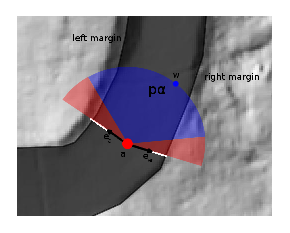
\includegraphics[width=\textwidth]{images/waypoint_new.eps}
    \caption{Selection of a waypoint: the skier $a$ selects the new waypoint $w$ choosing with uniform distribution on the angle $\delta\alpha$, a fraction of $\alpha$. The angle $\alpha$ is the angle between $e_{aR}$, the vector representing the direction towards the right edge, and $e_{aL}$, the vector towards the left edge,}\label{new_waypoint_pic}
  \end{center}
\end{figure}

A new waypoint is selected when the old waypoint is no longer feasible, meaning that it is not in the interval that the skier would consider when choosing a new waypoint, or when the skier has traveled more than $D$ meters after having chosen the last waypoint.

The new approach for waypoints selection considers closely skier speed and the effect of the slope shape on skier's action:\begin{enumerate}
\item \label{depending_velocity} Speed influences in two ways. 
\begin{itemize}
\item First, when skiers are faster they tend to turn more often, 
\item secondly, higher speed means higher frequency of waypoints selection.  
\end{itemize}
\item \label{frequency} of the selection of new waypoints should depend on the skiers speed, the more skiers are traveling fast, the more frequently they will choose new waypoints.
\item \label{depending_slope} The selection of a new waypoint should depend on the slope that the skier will face in his range of action: before flat areas skiers tend to go straight to increase velocity.

\item \label{avoid_impact} Skiers usually avoid to choose a direction that would make them turn right on the edge of the slope. Therefore, the new waypoint should be in a position that does not lead the skier to impact the edge of the slope.
\end{enumerate}

To fulfill the influences of skier's speed and shape of the slope it is possible to act on the parameter $\delta$ of the equation \ref{new_waypoint}. When $\delta$ is increasing, the width of the angle in which new waypoints can be chosen becomes larger. As a consequence the probability of performing turns becomes higher.

Point 1a \ref{depending_velocity} can be satisfied by making the parameter $\delta$ linearly depend on skier's speed $v$. Moreover it is required that when the speed $v$ is close to $0$ the width of the angle should be also close to $0$ and when $v$ is close to a high value of speed $v_{max}$ the angle should have maximum width. Therefore, $\delta$ can be set to
\begin{equation}\label{delta_vel}
\delta= \frac{v}{v_{max}}
\end{equation}

To fulfill the second requirement \ref{depending_slope} an additional factor depending on the slope should be considered. Let $s$ be the slope that the skier is going to encounter and let $s_{lim}$ a value of slope that is considered small enough to require an additional acceleration by the skier. Then if $s<s_{lim}$ the width of the angle in which to choose the new waypoint should be narrowed again. Taking into account \ref{delta_vel} then we can write $\delta$ as

\begin{equation}
\delta=\begin{cases}
   \frac{v}{v_{max}}\frac{s}{s_{lim}} & \text{if ($s < s_{lim}$)} \\
   \frac{v}{v_{max}} & \text{otherwise}
\end{cases}
\end{equation}
If, despite this, skiers will come to a complete stop (maybe due to a counter slope), they will have to move at constant speed.

The requirement \ref{frequency} is already met by the two  described above. In fact, since a new waypoint is chosen each time the skier has traveled more than $D$ meters, when a skier is faster he or she chooses waypoints more frequently.

Finally, to satisfy point \ref{avoid_impact} manipulating $\delta$ will  not be  enough. The minimum turning radius of skiers gives a bound to their ability of avoiding a collision or to hit the edges of the ski slope. Assuming that a skier do not choose a direction that will make them exit the ski slope, those angles indicating a direction along which the slope edge is reached in less than $R_{SC}$ meters are not considered in the selection of the waypoint.

\chapter{Implementation}\label{implementation}
The model was implemented using C++ and GRASS GIS. GRASS GIS is a Geographic Information System (GIS) open source software used for geospatial data management and analysis. It was chosen because it exposes its GIS engine in form of libraries that were used to perform the geospatial computation needed by the model.

\section{Technology choice}
Different technologies were explored to implement the GIS Backend needed by the model. The main technologies considered were PostGIS, QGIS, GDAL/OGR and GRASS GIS.

PostGIS is an open source spatial database extender for PostgreSQL database. It gives support for geographic objects manipulation allowing spatial queries to be run in SQL. The problem with PostGIS is that it does not have dedicate API for any language. It requires to use a PostgreSQL adapter (such as psycopg for python) and to build dynamically the queries in the chosen language. Moreover the raster data support is still immature in PostGIS.

Quantum GIS Desktop, also known as QGIS, is an open source GIS desktop application. QGIS supports both vector and raster formats. It have a module, PyQGIS, that supports scripting using the Python language. Unfortunately, the functionalities offered are more focused on spatial data visualization and do not give enough support for the analysis operations.

GDAL, Geospatial Data Abstraction Library, is an open source library for geospatial data translation and processing. The related library OGR Simple Feature Library provides a similar capability for simple vector data processing. GDAL exposes API for C,C++ and Python while the more widely used API for OGR are those for C++. OGR provides also slightly less complete API for C and Python API, although they are not really well documented. The problem using GDAL/OGR is especially the lack of support for the analysis of vector data: OGR offers useful API to read and write vector data, but analysis such as point linestring distance calculation are not available.

GRASS GIS, commonly referred to as GRASS (Geographic Resource Analysis Support System) is an open source GIS software that gives support for geospatial data management and analysis. To understand how GRASS API works it is necessary to look at the GRASS software structure (see Fig.\ref{grass_structure}. GRASS has a large GIS library, referred to as GRASS GIS Library, at the basis of the software stack. It is divided in two main library: the Raster File Processing library and the Vector File Processing library. It also contains many others library of less importance. The GRASS GIS Library is quite large and implements many basic GIS operation both for raster and vector format. The spatial data (both raster and vector) are stored in the GRASS map storage with the GRASS specific format. On the top of the GRASS GIS Library are built many modules for raster and vector processing. The modules perform analysis at a higher level, they are executables and they can be used from the GRASS GUI or from the command line.

\begin{figure}[!ht]
  \begin{center}
    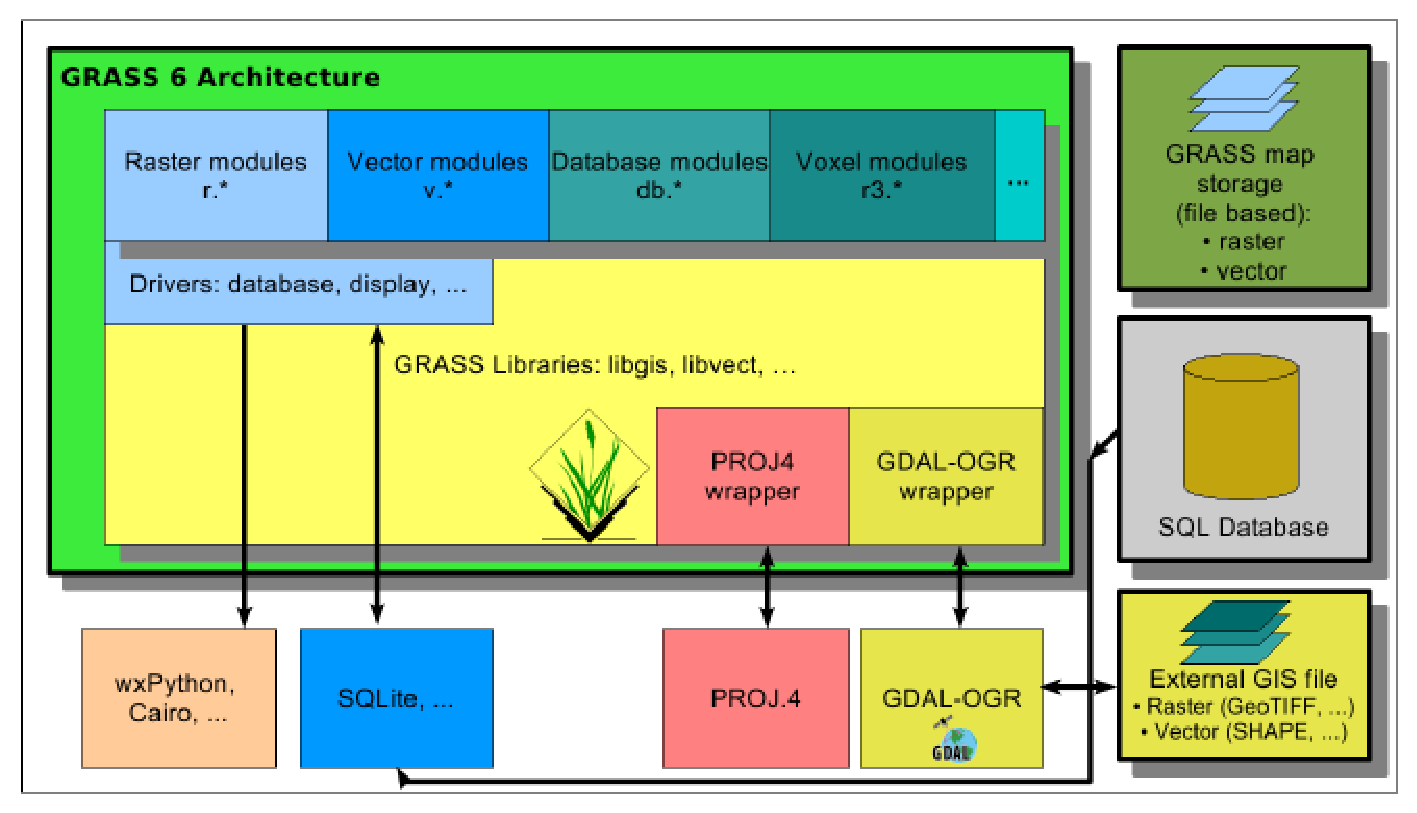
\includegraphics[width=\textwidth]{images/grass6_arch.eps}
    \caption{(from http://grass.osgeo.org} GRASS software architecture\label{grass_structure}
  \end{center}
\end{figure}

GRASS allows two basic levels of programming. The most simple approach is to use script programming to call the high-level GRASS modules. A more advanced approach is to access the low-level functionalities of the GRASS GIS library trough the C-API exposed. Since grass modules are executables, the first approach requires to spawn a new process each time a spatial computation is required. For the implementation of the model presented in \ref{model} this is not feasible. Even if the second approach forces the implementation to use GIS operations at a lower lever it has many advantages: it gives support for database routines (GRASS file management), projections, raster data management, area, line and point vector data management \cite{net2008} and it guarantees good performances.

GRASS GIS was chosen to implement the GIS Backend. Since the API is written in ANSI C, writing the code in C or in C++ has the advantage of accessing the API in a very simple manner. Moreover both C and C++ guarantee good performances and are often choose to implement this kind of simulation. C++ was preferred to C because it is object oriented. An object oriented design allows to better represent the concepts presented in the model, reducing the complexity and making the code structure clearer, and to keep the code more modular and flexible.

\section{Software structure}
The software structure was designed to be the most flexible as possible. The main entities modeled inside the software are the slope, the skiers and the forces. In Figure \ref{class_diagram} the class diagram of the software is described. The class Slope models the ski slope. It has a set of skiers, the skiers that are descending the slope, a set of physical forces, the physical forces that act on the slope and a set of social forces, the social forces skiers are subjected to. The Skier class models a skier: it has a position, a velocity, an acceleration and a status describing if is turning. The forces have been modeled with two different classes: the SocialForce class and the PhysicalForce class are abstract classes that act as base class respectively for all the social forces and for all the physical forces. Although the interface declared by this two classes is the same, they were not merged together because the two type of forces, social and physical, are conceptually different and in future development it is possible that changes in the model will require to have separated interfaces.

\begin{figure}[!ht]
  \begin{center}
    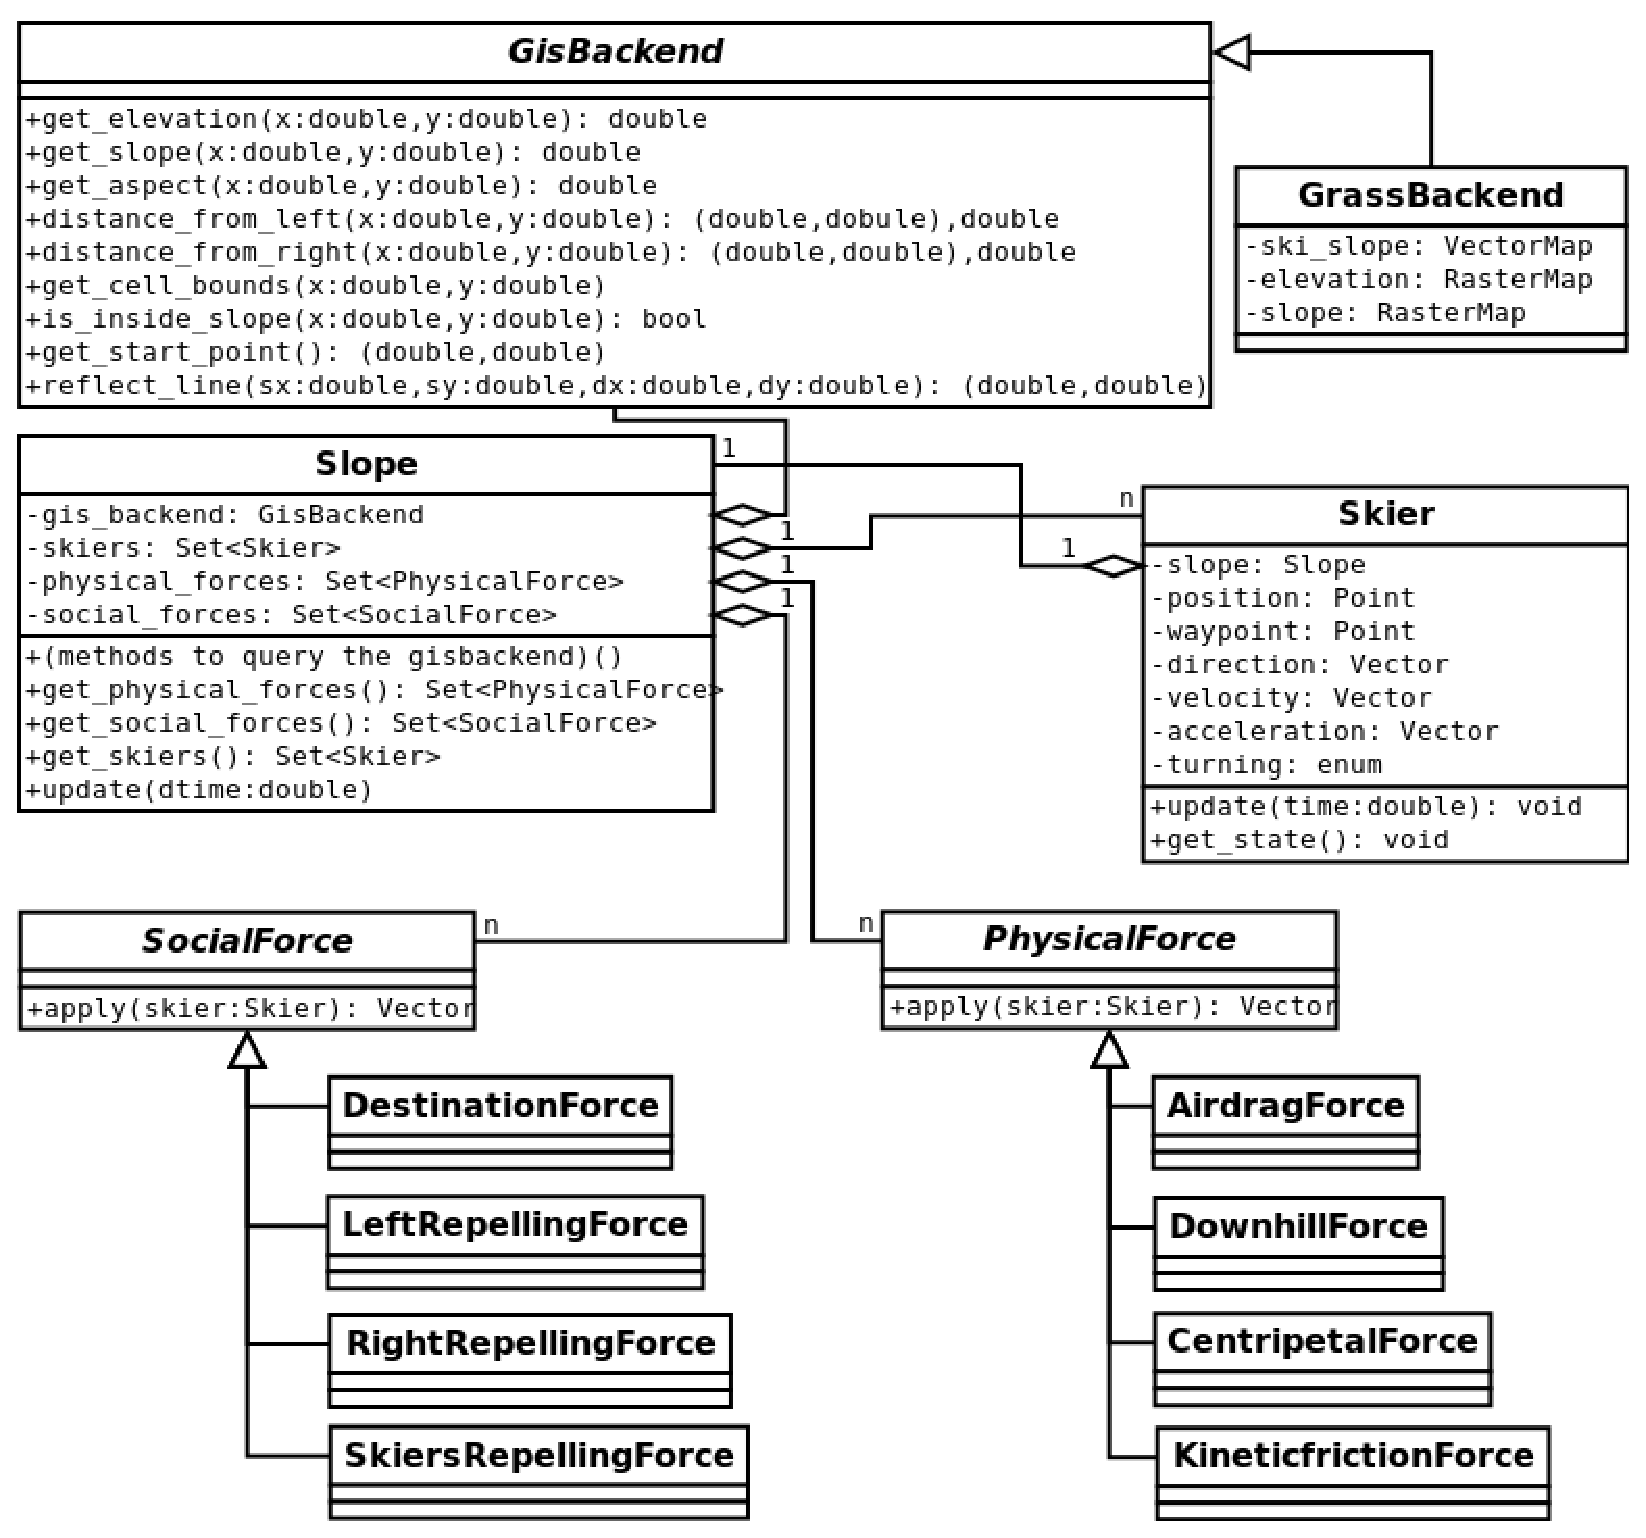
\includegraphics[width=\textwidth]{images/Class_diagram.eps}
    \caption{Class diagram}\label{class_diagram}
  \end{center}
\end{figure}

The simulation needs to perform some specific GIS computation. The implementation wanted to avoid dependency between the code related to the simulation and the code written to access the GRASS GIS library. In other words the implementation of the simulation should be independent by the technology chosen to implement the GIS Backend. For this reason, an abstract class called GisBackend was implemented. This class declares the interface that whatever GIS backend used to run the simulation should implement. This include methods to get elevation, slope and aspect for given coordinates, methods to get the distance of a point from the edges of the slope and the locations on the slope closer to the given point, methods to give random start points at the top of the ski slope and to determine if a given point is inside the ski slope and a method to reflect a line colliding on a slope edge.

The class GrassBackend implements the interface GisBackend and is the class actually used in the code when spatial computation are needed. The class GrassBackend perform the operations needed using the GRASS GIS Library. It requires to have available a DEM (Digital Elevation Model) raster map for the elevation, the slope and the aspect computation, a vector map with the polygon of the ski slope to determine if a point is inside the slope, a vector map with the lines of the right and left edges of the slope to find the distances from them and finally a vector map with the polygon of the start area and stop area to decide where skiers should be started and stopped.

\section{Input data}
The input data required by the simulation to run are the data needed by the GrassBackend. The Digital Elevation Model used was a Digital Terrain Model (DTM) of the area of Trentino. The DTM was obtained using the LIDAR technology, a remote sensing sensing technology that uses laser light to measures distances. The measurements were done in the years 2006 2007. It is at a resolution of 1x1m but for the area at high elevation the resolution is of 2x2m.

The measurements for the DTM were done in seasons without snow. As a consequence the DTM on which real skiers move is different from the DTM obtained with the Lidar. Two strategy was thought to simulate the effect of the snow on the DTM.

The first strategy uses a simple model to simulate the distribution of the snow. The model consider two limit cases to describe the profile of the snow. Given a surface $y(x)$ and a snowfall of $h$ meters. The first cases describes a new profile were the snow is supposed adhere perfectly to the terrain: $y_s(x)=y(x)+h$. The second cases consider the snow to behave like a liquid and create a new profile $y_L(x)$ where the new precipitation accumulates in the valleys making the profile constant and leaves $y_L(x)=y(x)$ on the ridges. Neither the first nor the second case can be considered realistic, but it can be thought that the real behavior of the snow can be described as an average between the two cases, so the actual profile after the precipitation can be described as
\begin{equation}
Y(x)=(1-l)y_s(x)+ly_L
\end{equation}
where $l$ is a parameter describing how much the snow has a behavior liquid-like. By the point of view of the implementation, the hard thing is to compute the profile $y_L$. For this purpose some GRASS modules was explored: r.watershed, r.terraflow, r.sim.water. The first two were excluded as they compute the flow accumulation rather than the water accumulation. The third modules, r.sim.water, is an overland flow hydrologic simulation based on path sampling method \cite{mit2004}. This module was used to compute the profile $y_L$.

The second strategy does not aim at building a realistic model for the snow precipitation but starts from the consideration that on a ski slope there are three main factors that determine the distribution of the snow: the snow precipitation, the snow produced by the snow cannons and the actions of the snow groomings. All this factors tend to smooth the original surface. To emulate this action the surface of the DTM is approximated with a smoothed surface. Starting from the original DTM raster map a vector map was produced where each original value of elevation were represented by a point. Then the GRASS module v.surf.rst was used to interpolate a new elevation map using regularized spline with tension \cite{mit2005}.

Figure \ref{profile_dtm} shows the profile of the original dtm, of the dtm obtained from the first strategy and of the dtm obtained from the second for a particularly critical point on a ski slope. The best result is given by the second strategy. The problem following the first strategy is the imprecision of the results from the module r.sim.water which does not returns a feasible profile for a liquid-like behavior. This can be due to a misconfiguration of the parameters of the module or maybe to a too demanding level of precision. Finally, the second strategy was chosen.

\begin{figure}[!ht]
  \begin{center}
    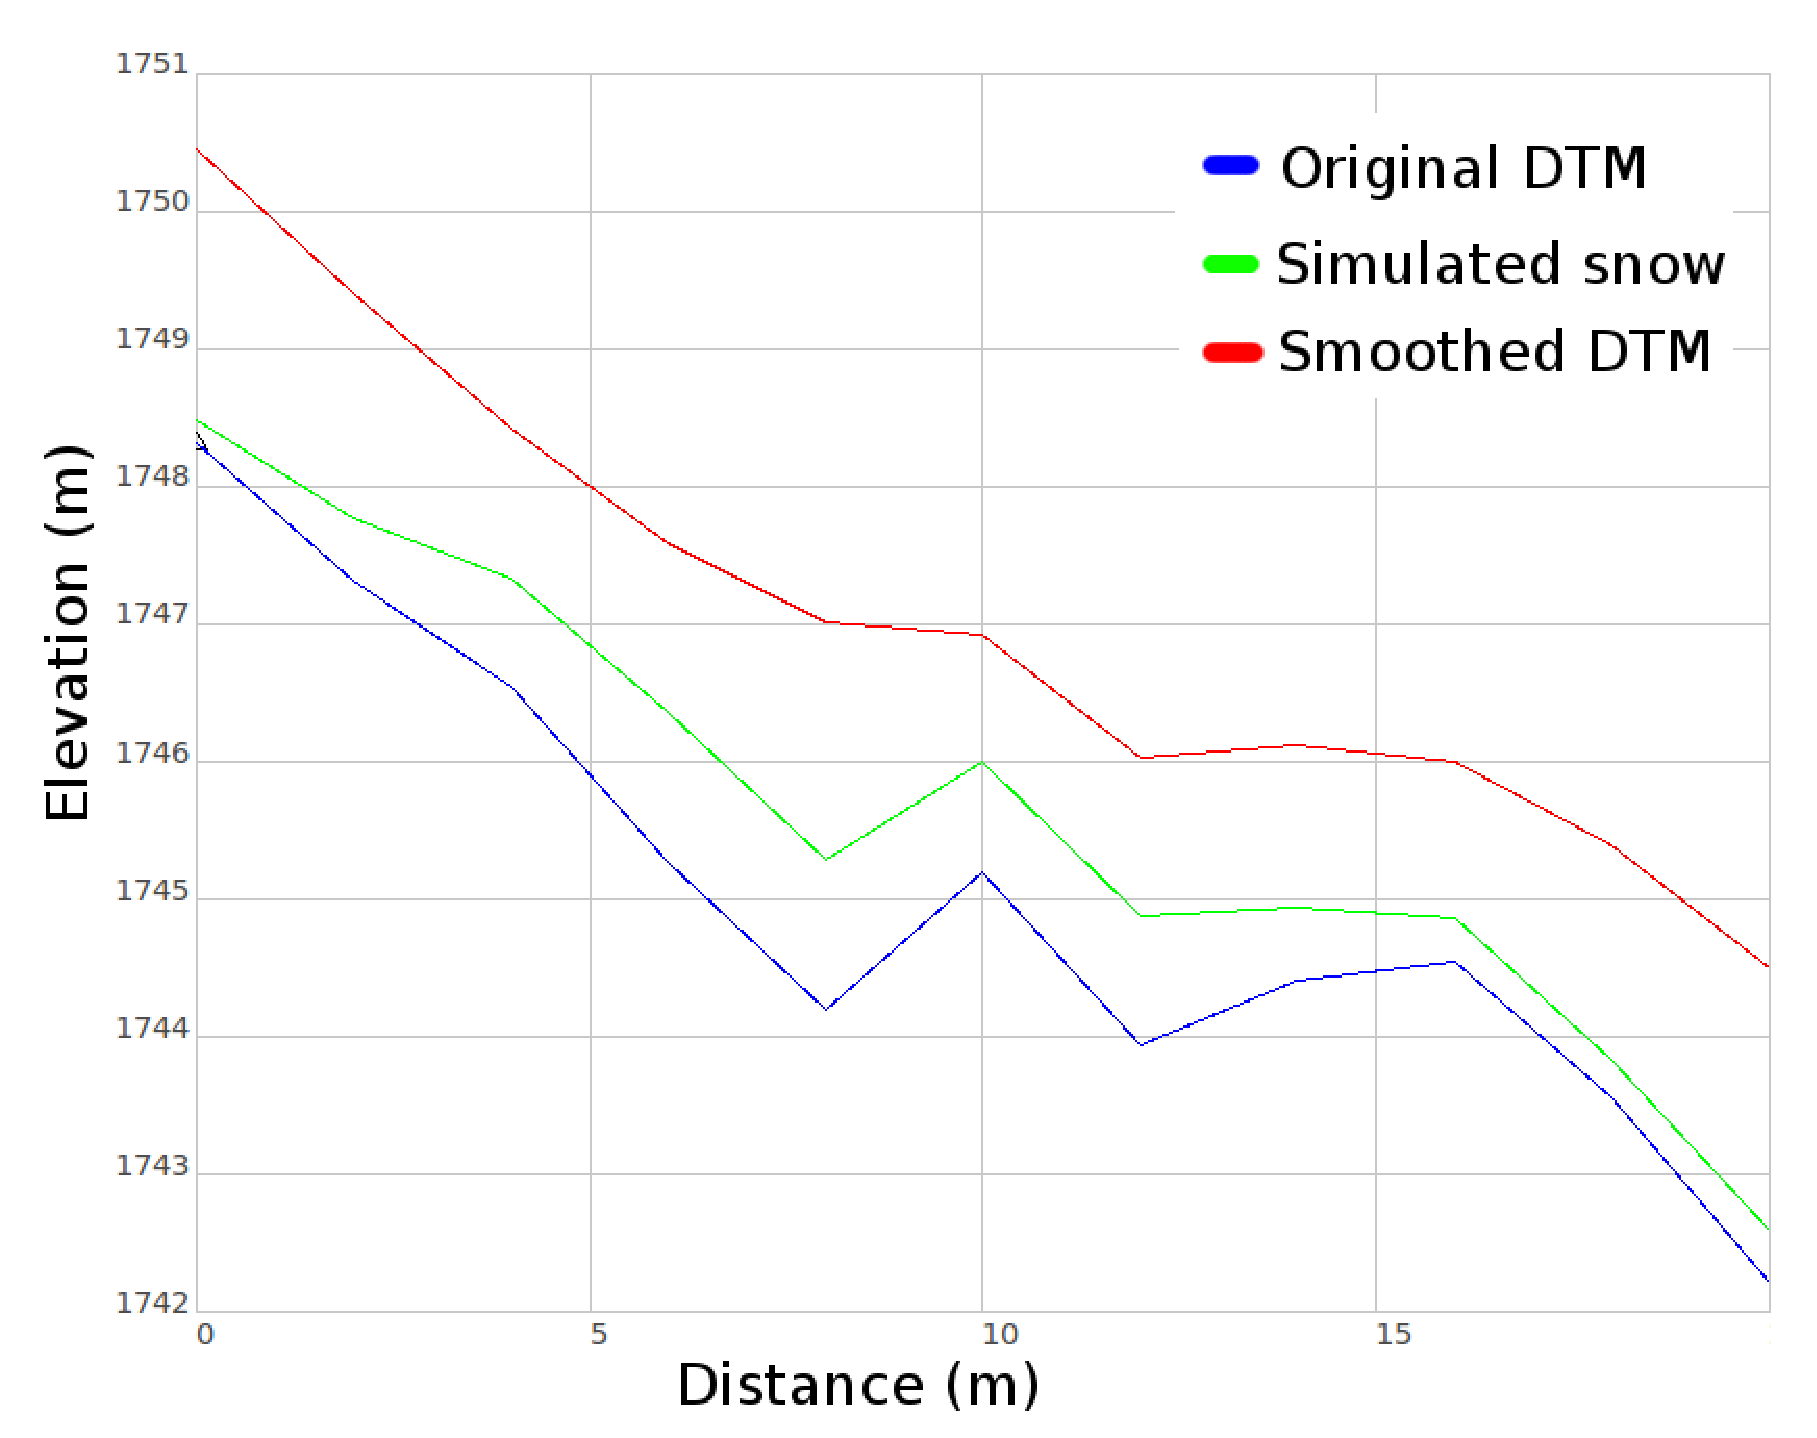
\includegraphics[width=0.7\textwidth]{images/profiles_dtm.eps}
    \caption{Profiles of the dtm and of the simulated dtm after rain fall}\label{profile_dtm}
  \end{center}
\end{figure}

Starting from the DTM slope raster map and aspect raster map are computed. The GRASS module r.slope.aspect was used. The slope raster map contains the slope, stated in degree of inclination from the horizontal. The slope of a cell is the maximum rate of change in value from that cell to its neighbors. Conceptually, computing the slope is equivalent to fits a plane to the z-value of a 3x3 neighborhood around the center cell. The slope value of this plane is computed using the average maximum technique(see. \cite{bur2009}). The direction the plan faces is the aspect.

The simulation requires to have in input the vector map with the polygon of the ski slope for which the model should be run. The ski slope (see. Fig.\ref{uno_tognola_3d} for an example) is extracted from a vector map containing the polygons of slopes of the skiing resort in Trentino. This data are available inside the SicurSkiWeb and were derived starting from orthophotos and tuned with measurements done in place. From the polygon of the ski slope left and right edge, start and stop areas are derived.

\begin{figure}[!ht]
  \begin{center}
    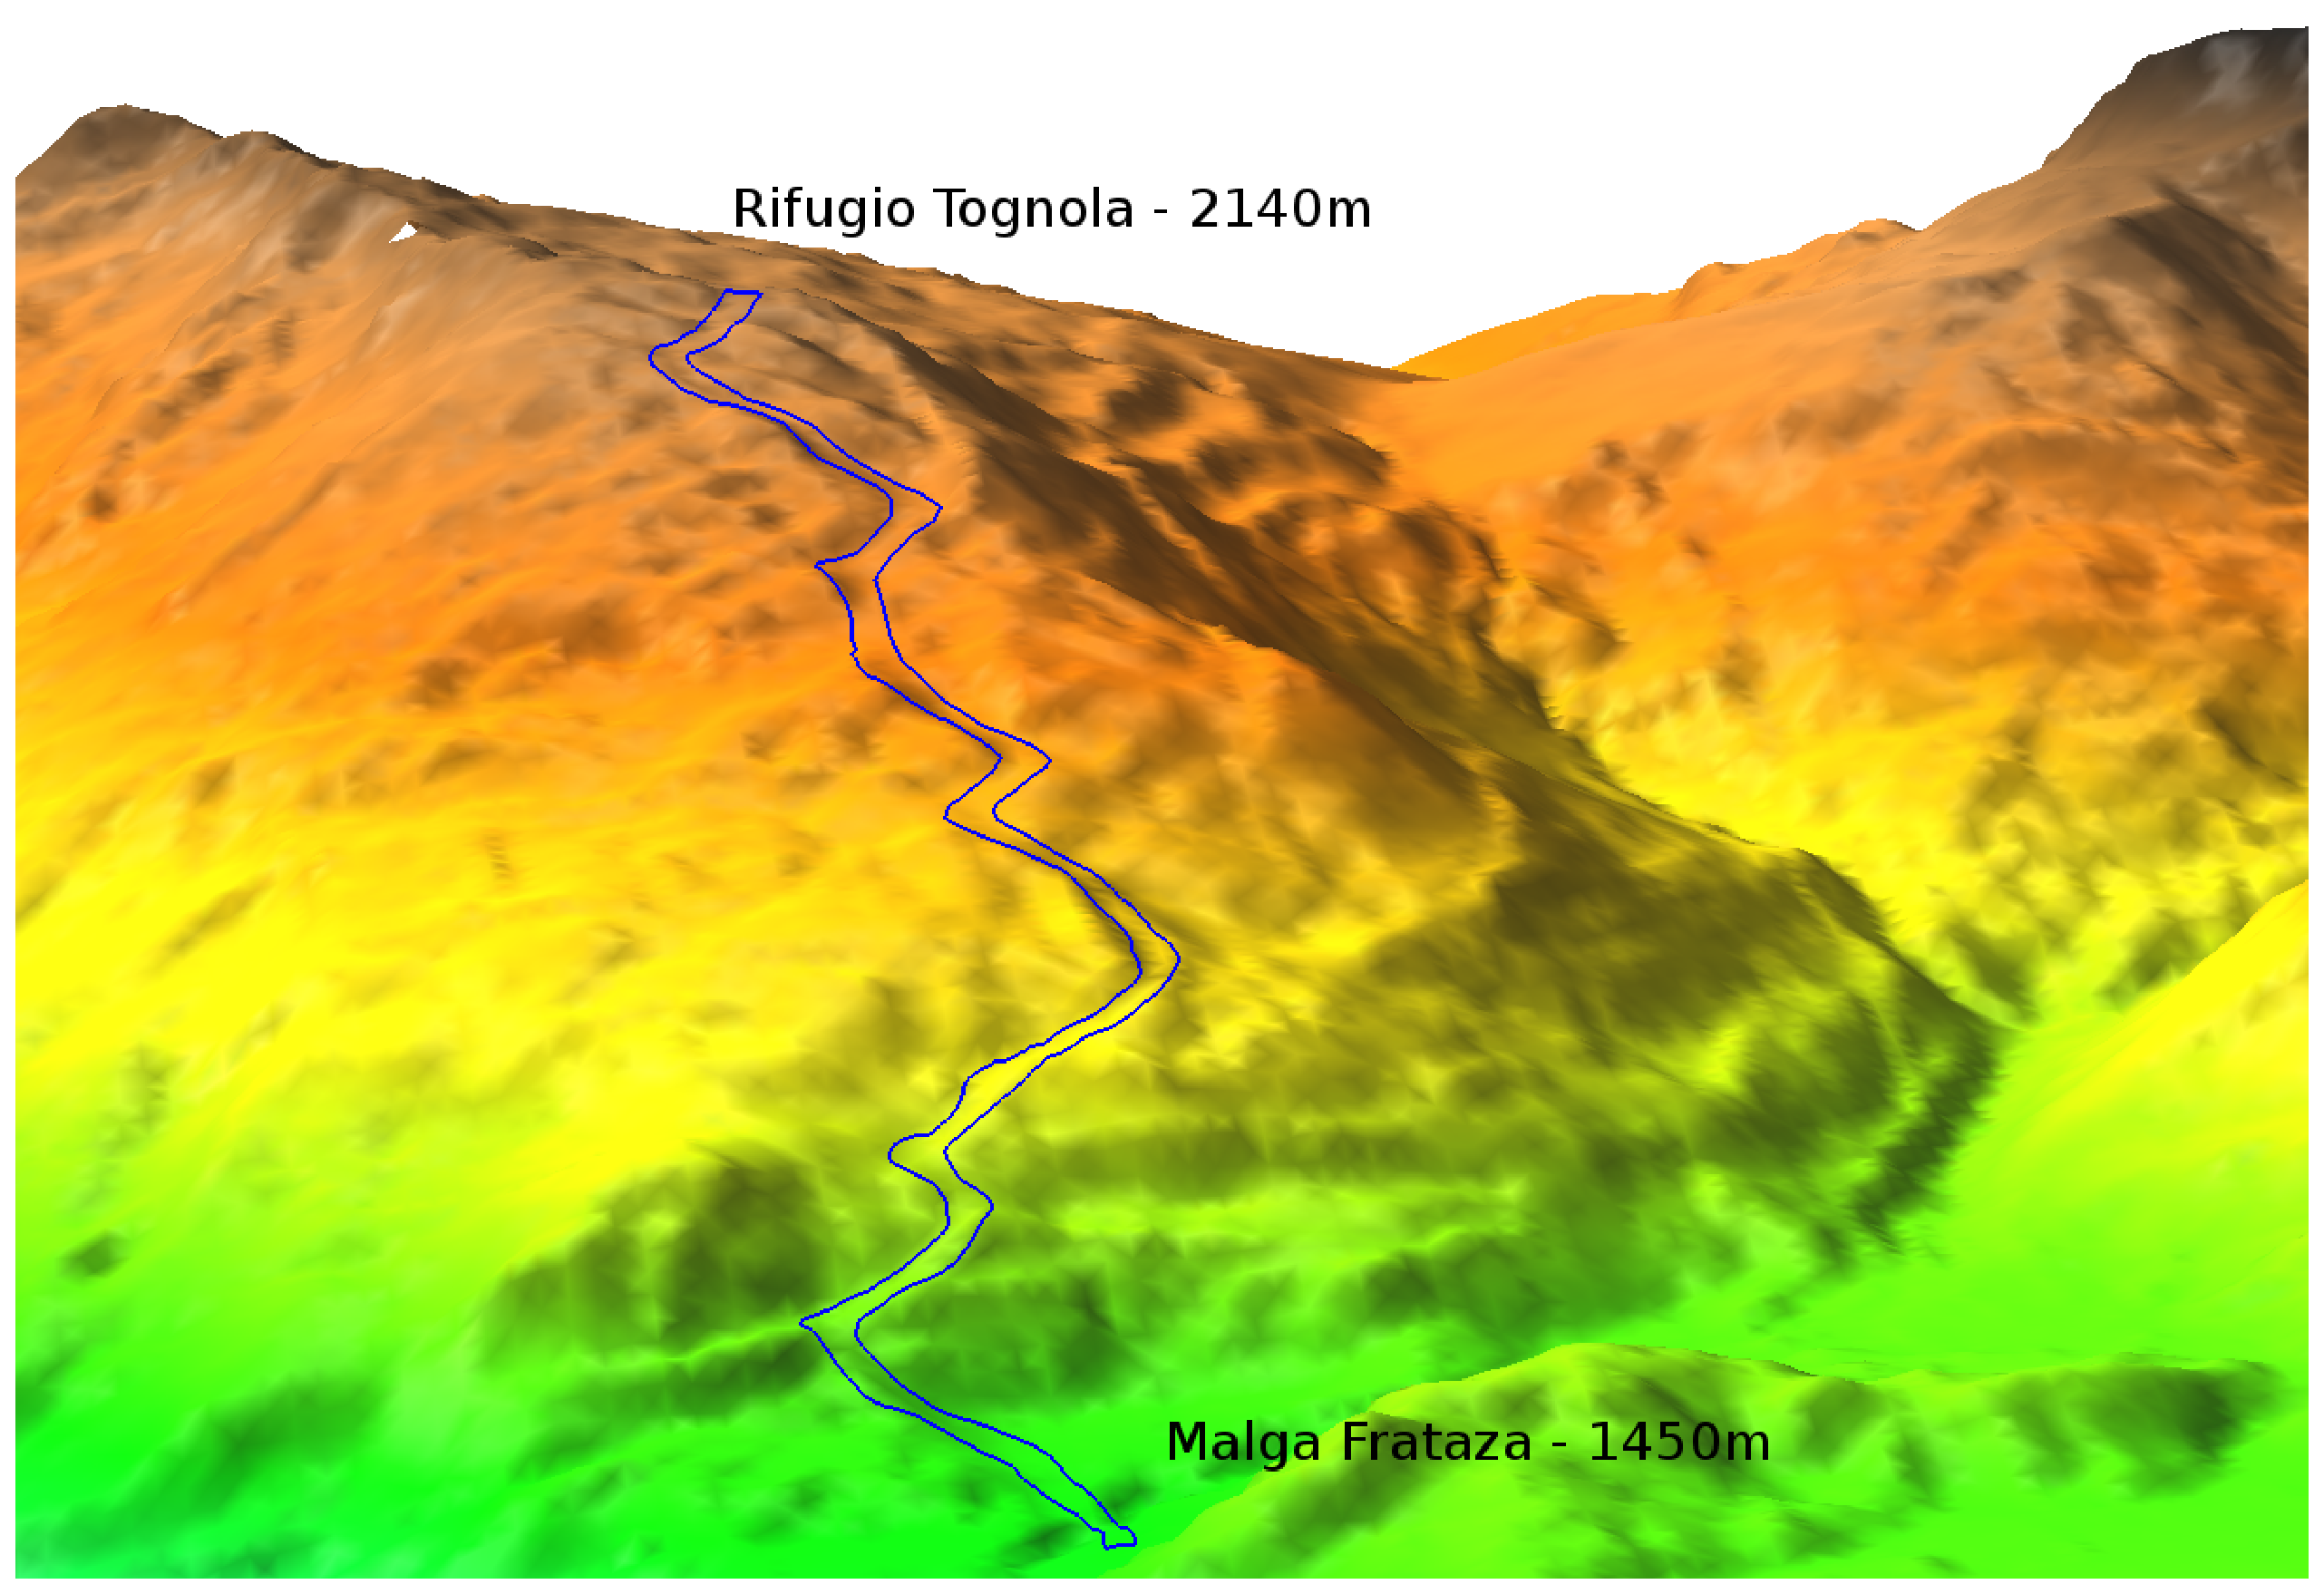
\includegraphics[width=\textwidth]{images/uno_tognola_3d.eps}
    \caption{3d visualization of the ski slope ``Uno di Tognola'' polygon (in blue) in San Martino di Castrozza.}\label{uno_tognola_3d}
  \end{center}
\end{figure}

\section{Output data}
The output produced by the simulation is a CSV file that log the skiers status at each moment of the simulation. The information reported for a time $t$ and a skier $a$ are the position $r_a$ and the velocity $\dot{r}_a$.

Starting from the csv two main analysis have been performed: speed average and average density of skiers computation. To analyze the speed of skiers along the ski slope a raster map of average speed has been produced. The map is obtained interpolating the value of speed produced by the simulation. The interpolation was done using the GRASS module v.surf.idw.


\section{Optimization}

parameters selection




\bibliography{thesis}
\end{document}
